%%%%%%%%%%%%%%%%%%%%%%%%%%%%%%%%%%%%%%%%%%%%%%%%%%%%%%%%%%%%%%%%%%%%
%% I, the copyright holder of this work, release this work into the
%% public domain. This applies worldwide. In some countries this may
%% not be legally possible; if so: I grant anyone the right to use
%% this work for any purpose, without any conditions, unless such
%% conditions are required by law.
%%%%%%%%%%%%%%%%%%%%%%%%%%%%%%%%%%%%%%%%%%%%%%%%%%%%%%%%%%%%%%%%%%%%

\documentclass[
  printed, %% This option enables the default options for the
           %% printed version of a document. Replace with `digital`
           %% to enable the default options for the digital version
           %% of a document.
  table,   %% Causes the coloring of tables. Replace with `notable`
           %% to restore plain tables.
  lof,     %% Prints the List of Figures. Replace with `nolof` to
           %% hide the List of Figures.
  lot,     %% Prints the List of Tables. Replace with `nolot` to
           %% hide the List of Tables.
  %% More options are listed in the user guide at
  %% <http://mirrors.ctan.org/macros/latex/contrib/fithesis/guide/mu/fi.pdf>.
]{fithesis3}

%% The following section sets up the locales used in the thesis.
\usepackage[
  main=slovak, %% By using `czech` or `slovak` as the main locale
               %% instead of `english`, you can typeset the thesis
               %% in either Czech or Slovak, respectively.
  slovak, english %% The additional keys allow
]{babel}          %% foreign texts to be typeset as follows:
				  %%  \begin{otherlanguage}{english}  ... \end{otherlanguage}

\usepackage{paratype}

%% The following section sets up the metadata of the thesis.
\thesissetup{
    date          = \the\year/\the\month/\the\day,
    university    = mu,
    faculty       = fi,
    type          = mgr,
    author        = Matej Majdiš,
    gender        = m,
    advisor       = doc. RNDr. Vlastislav Dohnal\, Ph.D.
    title         = {Rozpoznanie užívateľa na základe informácií o HTTP komunikácií},
    TeXtitle      = {Rozpoznanie užívateľa na základe informácií o HTTP komunikácií},
    keywords      = {keyword1, keyword2, ...},
    TeXkeywords   = {keyword1, keyword2, \ldots},
}

\thesislong{abstract}{
	TODO

}

\thesislong{thanks}{
	TODO
}

%% The following section sets up the bibliography.
\usepackage{csquotes}
\usepackage[              %% When typesetting the bibliography, the
  backend=biber,          %% `numeric` style will be used for the
  style=numeric,          %% entries and the `numeric-comp` style
  citestyle=numeric-comp, %% for the references to the entries. The
  sorting=none,           %% entries will be sorted in cite order.
  sortlocale=auto         %% For more unformation about the available
]{biblatex}               %% `style`s and `citestyles`, see:
%% <http://mirrors.ctan.org/macros/latex/contrib/biblatex/doc/biblatex.pdf>.
\addbibresource{example.bib} %% The bibliograpic database within
                          %% the file `example.bib` will be used.
                          
\usepackage{makeidx}      %% The `makeidx` package contains
\makeindex                %% helper commands for index typesetting.

%% These additional packages are used within the document:
\usepackage{paralist}
\usepackage{amsmath}
\usepackage{amsthm}
\usepackage{amsfonts}
\usepackage{url}
\usepackage{menukeys}
\usepackage{float}
\usepackage[plainpages=false, pdfpagelabels]{hyperref}

\begin{document}

\chapter{Úvod}
Problematika jednoznačnej identifikácie používateľa je dnes veľmi
dôležitou a riešenou témou. Jedným z hlavných dôvodov je fakt, že väčšina
dnešných existujúcich, prípadne novo vznikajúcich systémov a aplikácií je
nejakým spôsobom zapojená do Internetu. Zároveň zaznamenávame nárast
aplikácií, ktoré poskytujú užívateľom webové rozhranie a ústup takzvaných
desktopových aplikácií.

\begin{figure}[h]
  \centering
    
\includegraphics[width=.80\textwidth]{images/web-vs-desktop.png}
  \caption{Vizualizácia pomeru počtu užívateľov webových a desktopových
  aplikácií v čase, zdroj: vlastné spracovanie}
  \label{fig:web-vs-desktop}
\end{figure}

	Z tohto vyplýva potreba rozoznania a identifikácie používateľov, ktorý s
danou aplikáciou interagujú. Existuje niekoľko rôznych prístupov k 
identifikácií, od mapovania IP adries sieťovej vrstvy až po aplikačnú správu
užívateľských účtov. Podrobne sa nimi zaoberá kapitola \ref{ch:existing}.
Cieľom tejto práce je vytvoriť unikátny identifikátor na základe informácií
dostupných z \textit{HTTP} protokolu. Pred zostavením samotného algoritmu je
preto dôležité popísať niektoré kľúčové oblasti a postupy.

Nasledujúce kapitoly sa preto budú stručne zaoberať fungovaním aplikácií typu
klient-server, modelom sieťových vrstiev či útokmi typu \textit{Denial of
Service}. Ďalej v práci popíšem spomínané existujúce prístupy a vlastný návrh
algoritmu identifikácie užívateľa. 

\section{Aplikácie typu Klient-Server}
	S pokračujúcim vývojom nových technológií sa Web stáva stále väčšou
súčasťou našich životov. Web taktiež už nie je limitovaný prehliadaním na
počítačoch. Musí sa prispôsobovať rôznym novým technológiám, ako sú napríklad
mobilné, či iné zriadenia. Najčastejšie používaným modelom komunikácie pre
architektúru webových aplikácií je tzv. Klient-Server model. Základnou
myšlienkou tohto modelu je zaslanie požiadavku (\textit{requestu}) klientom na
server, ktorý vystupuje ako poskytovateľ služby.

\begin{figure}[h]
  \centering
    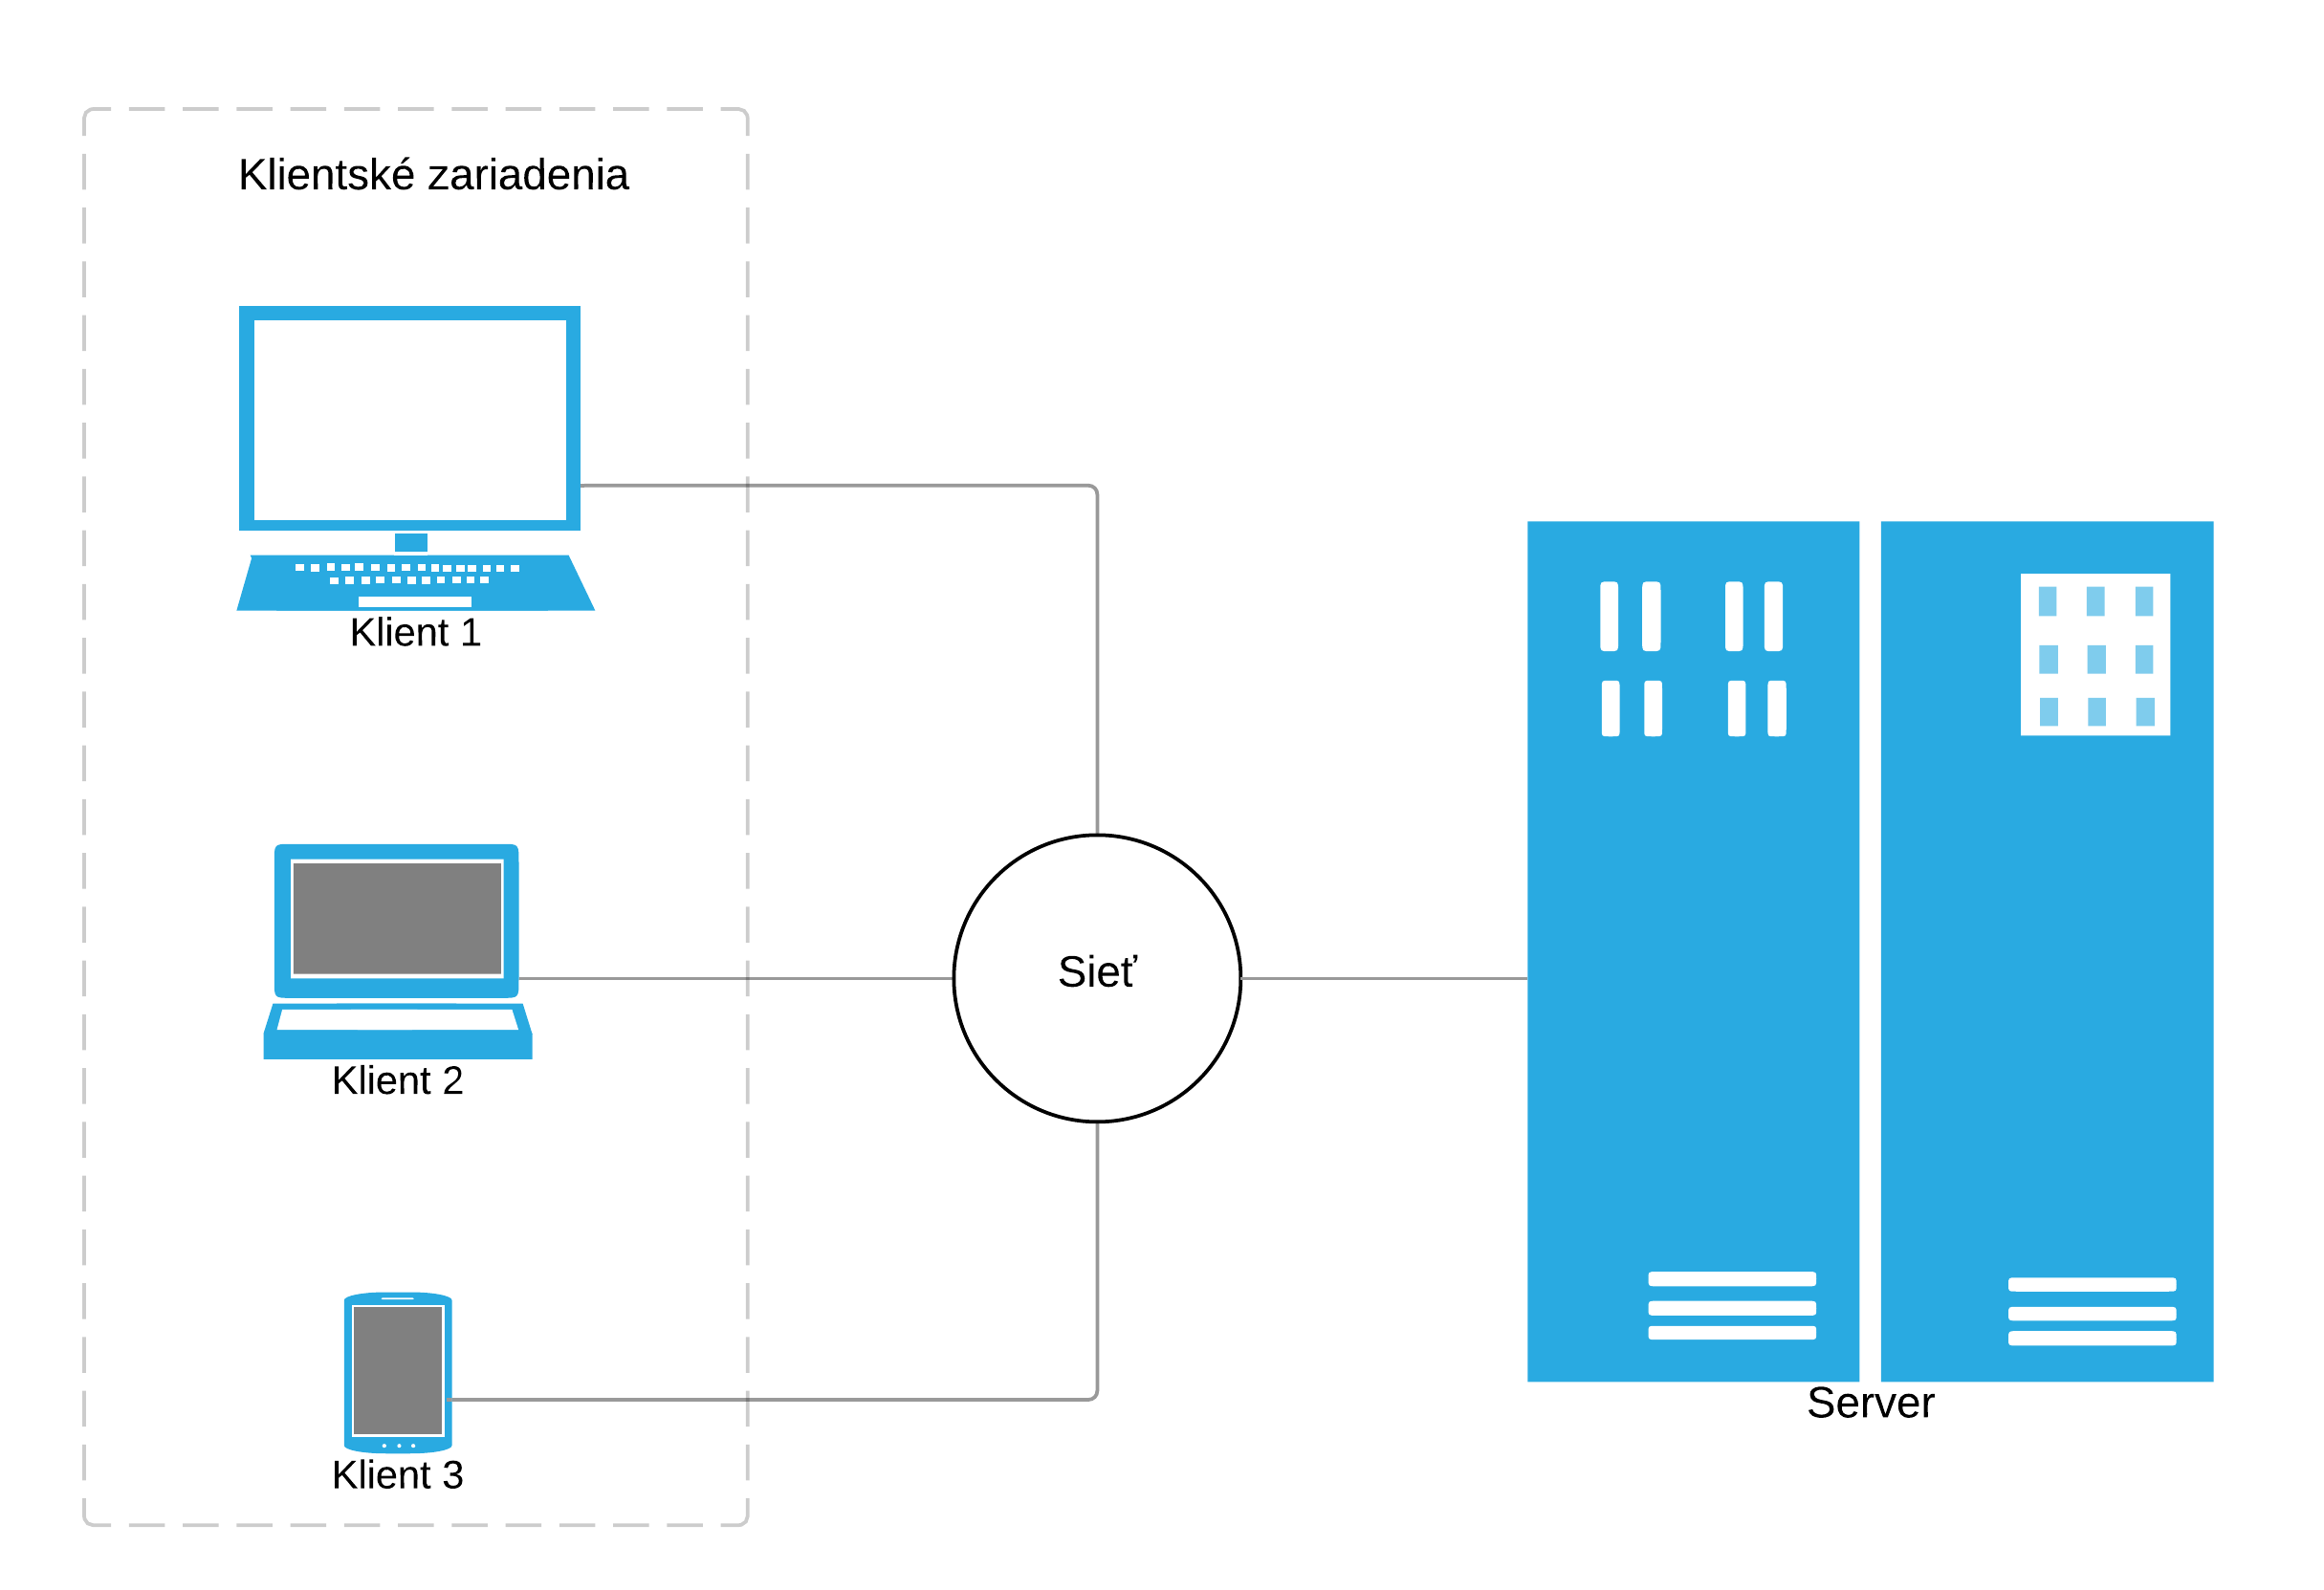
\includegraphics[width=.99\textwidth]{images/C-S-basic.png}
  \caption{Schéma znázorňuje základnú architektúru modelu Klient-Server, zdroj:
  vlastné spracovanie}
  \label{fig:cs-basic}
\end{figure}

\subsection{Klient-Server model}
Pretože Klient-Server model je používaný rôznymi typmi aplikácií bolo nutné
použiť štandardizované protokoly, na základe ktorý ch bude možné komunikovať.
Základné používané protokoly sú: \textit{FTP (File Transfer Protocol)},
\textit{Simple Mail Transfer Protocol (SMTP)} a \textit{Hypertext Transfer
Protocol (HTTP)}. Bližšie sieťové vrstvy a jednotlivé protokoly popisuje
kapitola \ref{ch:net-layers}.

\subsection{Architektúra}
Architektúra modelu Klient-Server sa vo všeobecnosti typicky skladá z troch 
častí:
\begin{itemize}
	\item Aplikačný server
	\item Databázový server
	\item Zariadenie klienta
\end{itemize}
Zároveň Existujú dva základné typy architektúr: 
\begin{itemize}
	\item 2-stupňová \textit{(2-tier)}
	\item 3-stupňová \textit{(3-tier)}
\end{itemize}

\textit{2-tier} architektúra zahrna len zariadenie klienta a databázový server.
U tohoto typu architektúry je aplikácia spustená na zariadení klienta, ktoré sa
následne pripája priamo na server. Zariadenie tak obsluhuje zároveň
\textit{business} logiku aj zobrazovanie aplikácie. Inak tento typ architektúry
nazývame aj tučný klient(\textit{thick client}).

\begin{figure}[H]
  \centering
    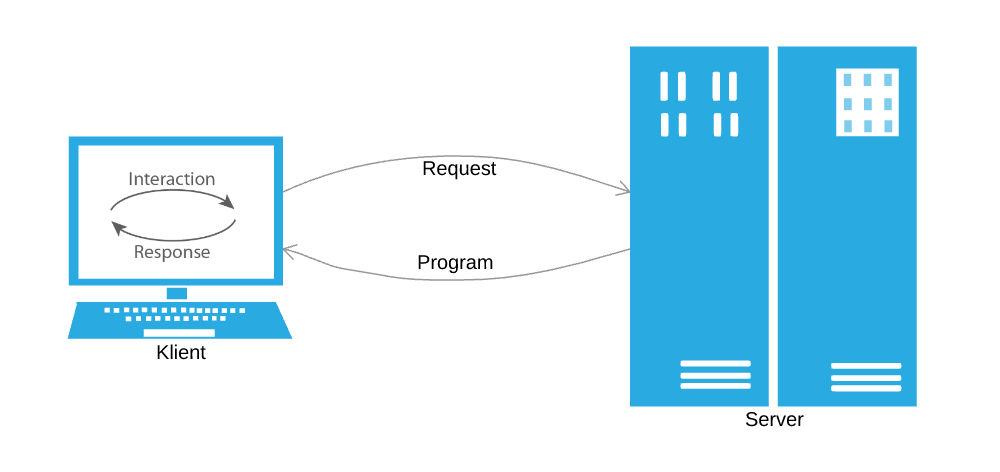
\includegraphics[width=\textwidth]{images/C-S-thick.png}
  \caption{Grafické znázornenie a popis priebehu komunikácie 2-tier architektúry,
  zdroj: vlastné spracovanie}
  \label{fig:cs-thick}
\end{figure}

\textit{3-tier} architektúra, ktorou sa budem zaoberať v tejto práci sa od
\textit{2-tier} líši najmätým, že okrem zariadenia klienta a databázového servera
zahŕňa aj aplikačný server. Tento je následne používaný na obsluhu
\textit{business} logiky aplikácie a komunikáciu s databázou, pričom zariadenie
klienta slúž len na zobrazovanie. Iný názov pre takýto typ architektúry je tenký
klient (\textit{thincient}).

\begin{figure}[H]
  \centering
    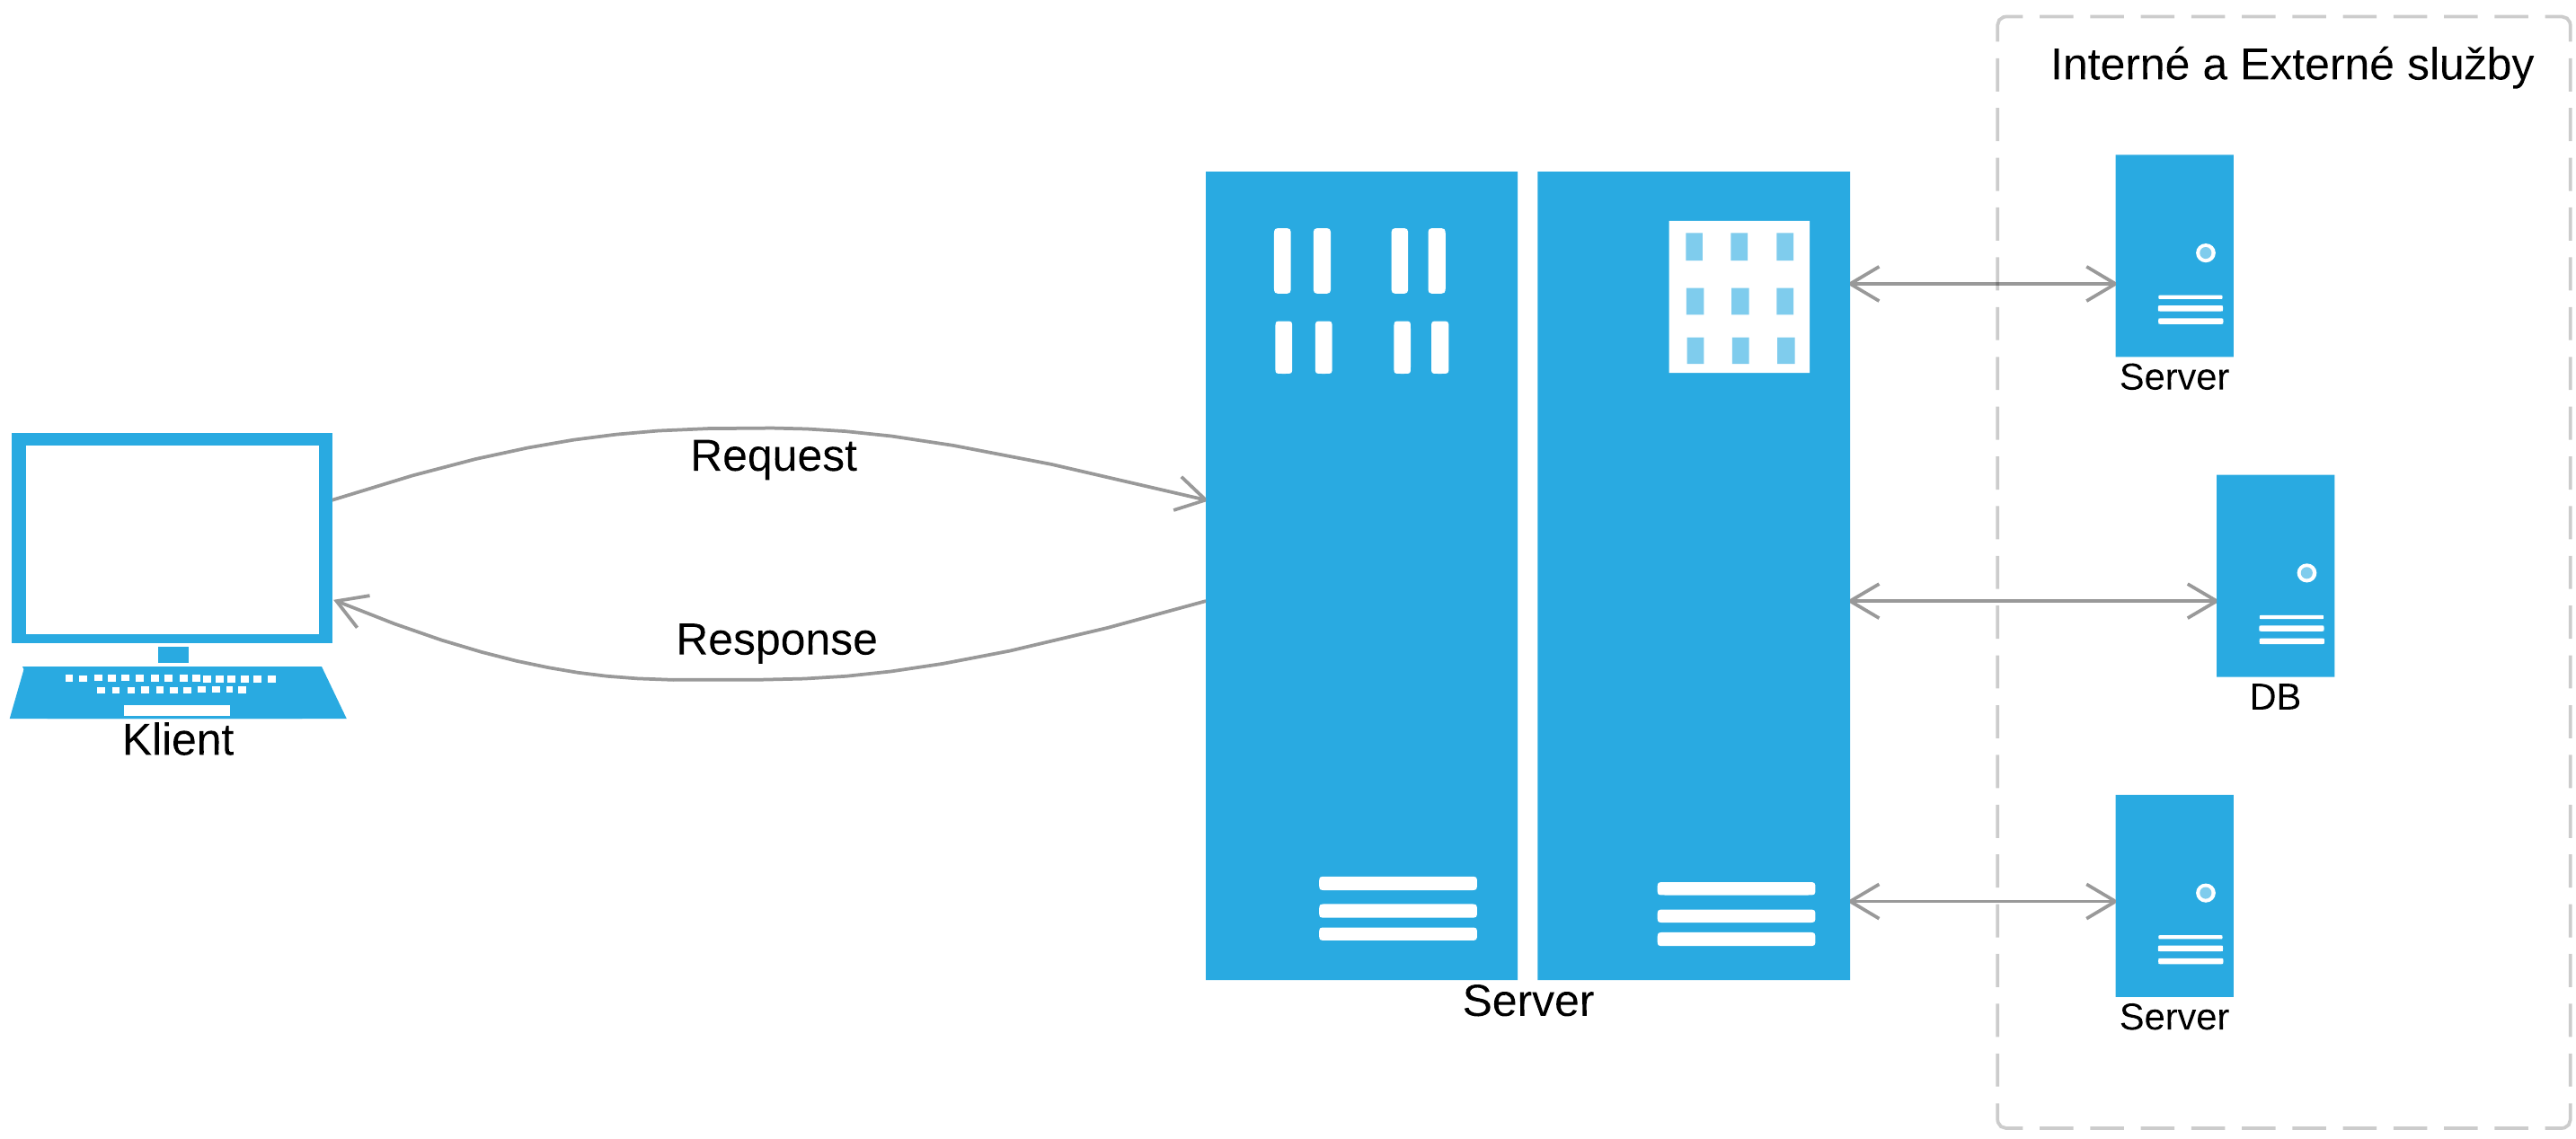
\includegraphics[width=\textwidth]{images/C-S-thin.png}
  \caption{Grafické znázornenie a popis priebehu komunikácie 3-tier architektúry,
  zdroj: vlastné spracovanie}
  \label{fig:cs-thin}
\end{figure}

Nasledujúce kapitoly tejto práce sa budú zaoberať jedným z najdôležitejších
problémov Webových aplikácií, ktorým je identifikácia užívateľa. Najskôr kapitola
\ref{ch:net-layers} popisuje jednotlivé sieťové vrstvy a protokoly, ktorých
informácie je možné použiť ka následnej identifikácií. Ďalšou časťou je zhrnutie
existujúcich prístupov k rozoznaniu užívateľov v kapitole \ref{ch:existing} a 
popis útokov typu DOS v kapitole \ref{ch:dos}. Najdôležitejšou časťou je však
samozrejme kapitola \ref{ch:footprint}, ktorá popisuje návrh samotného 
algoritmu identifikátoru.

\chapter{Sieťové vrstvy}
\label{ch:net-layers}
Nasledujúca kapitola stručne popisuje jednotlivé sieťové vrstvy TCP/IP modelu a
ich protokoly. Zameriava sa na štruktúry a informácie, ktorých pochopenie je
dôležité pre ďalšie zložky teoretickej a praktickej časti práce. Ide najmä o
konkrétne informácie jednotlivých protokolov skutočne použité v implementácií
identifikačného algoritmu.

\begin{figure}[h]
  \centering
    
\includegraphics[width=.80\textwidth]{images/net-layers.png}
  \caption{Vizualizácia vrstiev TCP/IP modelu, jeho najpoužívanejších protokolov
  a prenosových štruktúr, zdroj: vlastné spracovanie}
  \label{fig:net-layers}
\end{figure}

\section{Aplikačná vrstva}
Na vrchole hierarchie je Aplikačná vrstva abstrakciou, ktorá špecifikuje
konkrétne protokoly a metódy používané hostiteľskými uzlami v sieti. Táto
vrstva je definovaná jednak v TCP/IP ale aj OSI
\textit{(Open Systems Interconnection)} modele sieťovej komunikácie.

Táto práca narába s modelom TCP/IP, v ktorom aplikačná vrstva definuje práve
protokoly a metódy rozhraní pre komunikáciu medzi jednotlivými procesmi
spájaných strán v sieti. Samotná aplikačná vrstva však len štandardizuje formu
komunikácie, pri čom ustálenie uceleného dátového spojenia a správu prenosu dát
u aplikácií typu klient-server a \textit{peer-to-peer} ponecháva na protokoloch
nasledujúcej - transportnej vrstvy. Keďže aplikačná vrstva nijakým spôsobom
nepopisuje a nešpecifikuje konkrétne pravidlá pre formu prenášaných dát,
aplikácie samotné musia obsahovať logiku, ktorá zabezpečí, že obe komunikujúce
strany budú v tomto ohľade navzájom kompatibilné.

Aplikačná vrstva definuje veľké množstvo protokolov, ako napríklad:
\begin{itemize}
	\item HTTP/HTTPS
	\item TLS/SSL poskytujúci zabezpečenú vzdialenú komunikáciu po sieti
	\item FTP využívaný na prenos súborov
	\item SMTP určený pre emailovú komunikáciu
	\item DNS realizujúci systém hierarchie doménovým mien, a iné...
\end{itemize}
Pri tvorbe identifikátoru sa však budeme venovať najmä informáciám z protokolov
rodiny HTTP, konkrétne teda hlavičkám a atribútom HTTP a HTTPS.

\subsection{HTTP}
HTTP \textit{(Hypertext Transfer Protocol)} je distribuovaný protokol určený
pre spoluprácu a prenos informácií medzi jednotlivými systémami určenými na
prácu s hyper-médiami. Tento protokol je bez-stavový a vo všeobecnosti
použiteľný nielen pre prenos hypertextu, ale aj správu DNS serverov, prípadne
zložitejších objektov a systémov, v ktorých uplatní rozsiahlu škálu svojich
hlavičiek a chybových hlášok. Charakteristickým znakom tohto protokolu je aj
možnosť voľby reprezentácie dát, čo dáva systémom veľkú nezávislosť na
prenášanom formáte.

HTTP funguje na princípe požiadavku a odpovede \textit{(request - respone)}
založenom na fungovaní samotného klient-server modelu. Klientom môže byť
napríklad webový prehliadač, serverom zasa aplikácia spustená na počítači
hostiteľského uzla. V tomto prípade teda webový prehliadač zašle správu vo
forme HTTP požiadavku na server. V ideálnom prípade server tento požiadavok
\textit{(request)} spracuje a vygeneruje odpoveď (napríklad HTML stránku),
ktorú vráti klientovi ako správu vo formáte HTTP odpovede \textit{(response)}.
Odpoveď pre klienta vždy obsahuje takzvaný \textit{(status)}, ktorý informuje o
dokončení požiadavku a prípadne samotné telo so správou odpovede.

Celá relácia HTTP spojenia medzi dvoma uzlami je teda sekvenciou niekoľkých
takýchto \textit{(request - respone)} transakcií. Samotný prenos dát však nie
je realizovaný na úrovni HTTP protokolu, ale prostredníctvom protokolu TCP
na úrovni transportnej vrstvy. HTTP Klient iniciuje ustálenie TCP spojenia pre
špecifický port serveru (typickými portmi sú 80, 443 alebo 8080). HTTP server
počúva na danom porte a čaká na správu požiadavku klienta. Po prijatí správy ju
už server štandardne spracuje a vráti odpoveď. 

Klient a server komunikujú prostredníctvom zasielanie plain-textových správ.
Požiadavok pozostáva z nasledujúcich informácií: 
\begin{itemize}
	\item Definícia požiadavku
	\item HTTP hlavičky (napríklad: \textit{Accept-Language: en})
	\item Prázdny riadok
	\item Prípadné telo správy
\end{itemize}

Takisto správa odpovede má definovaný formát podobný formátu požiadavku, ktorý
sa skladá z nasledujúcich položiek:
\begin{itemize}
	\item Status spracovania požiadavku a dôvod
	\item HTTP hlavičky odpovede (napríklad: \textit{Content-Type: text/html})
	\item Prázdny riadok
	\item Prípadné telo správy odpovede
\end{itemize}

Prvý riadok definície a každá z hlavičiek musia byť zakončené znakmi
\textit{<CR><LF>}
(znak pre \textit{carriage return} nasledovaný znakom \textit{line feed}).
Prázdny riadok musí zároveň pozostávať výlučne zo znakov \textit{<CR><LF>}.
Z pohľadu identifikácie budú neskôr veľmi dôležité práve HTTP hlavičky. U HTTP
verzie 1.1 je jedinou povinnou hlavičkou \textit{Host} definujúci server, na
ktorý bol požiadavok odoslaný.

\begin{figure}[h]
  \centering
    
\includegraphics[width=.80\textwidth]{images/net-http.png}
  \caption{Príklad štruktúry HTTP požiadavku a odpovede}
  \label{fig:net-http}
\end{figure}

\section{Transportná vrstva}
V kontexte TCP/IP modelu sieťovej komunikácie sa transportná vrstva nachádza
ako druhá v poradí medzi aplikačnou a sieťovou vrstvou. Ide o súbor protokolov
a metód, ktoré poskytujú takzvanú \textit{host-to-host} komunikáciu
jednotlivých sieťových uzlov protokolom vyššie popísanej aplikačnej vrstvy.
Konkrétne implementuje funkcionalitu samotného prenosu dát v dátovom toku,
zabezpečuje jeho spoľahlivosť, riadenie a multiplexovanie. 

Medzi najznámejšie protokoly tejto vrstvy patrí napríklad TCP
\textit{(Transmission Control Protocol)}, ktorého názov nesie aj samotný
sieťový model. Tento protokol je orientovaný na prenos zložitejších spojení,
naproti čomu druhý z protokolov - UDP \textit{(User Datagram Protocol )} je
vhodný a používaný skôr pre jednoduchšie správy a spojenia. Protokol TCP je
komplexnejší najmä kvôli svojmu návrhu, ktorý uchováva stav jednotlivých
transakcií a zabezpečuje spoľahlivosť doručenia dátových správ. Ďalšími
významnými protokolmi transportnej vrstvy sú DCCP
\textit{(Datagram Congestion Control Protocol)} využívaný napríklad pri prenose
multimédií, alebo SCTP \textit{(Stream Control Transmission Protocol)}, ktorý
sa zaoberá prenosom telefónnej signalizácie.

\subsection{Protokol TCP}
TCP je jeden z najdôležitejších a najpoužívanejších protokolov celého sieťového
modelu. Pracuje s ním množstvo ďalších protokolov aplikačnej vrstvy ako
napríklad: HTTP, FTP alebo POP3. Jeho najdôležitejšou charakteristikou je
pravdepodobne garancia kompletného doručenia všetkých paketov v správnom
poradí. K samotným dátam aplikačnej vrstvy preto TCP pripája ku každému paketu
aj takzvanú TCP hlavičku \textit{TCP Header}, ktorá ho dopĺňa o informácie
potrebné pre dosiahnutie tejto funkcionality.

\begin{figure}[h]
  \centering
    
\includegraphics[width=.80\textwidth]{images/net-tcp-head.png}
  \caption{Schéma popisujúca štruktúru TCP hlavičky a informácií, ktoré sú v
  nej uložené}
  \label{fig:net-tcp-head}
\end{figure}

Niektoré informácie týchto hlavičiek sú využívané jednak u existujúcich
nástrojov na identifikáciu užívateľov, ktorým sa podrobne venuje kapitola
\ref{ch:existing}. Ich vyžitie v algoritme identifikátoru tejto práce následne
popisuje kapitola \ref{ch:footprint}.

Aby mohlo dôjsť k samotnému odoslaniu požadovaných dát, musí byť medzi klientom
a hostiteľom ustálené TCP spojenie. Ustálenie aj ukončenie tohto spojenia má
presne definovanú formu komunikácie nazývanú \textit{three-way handshake}, ktorú
popisuje nasledujúci diagram.

\begin{figure}[h]
  \centering
    
\includegraphics[width=.80\textwidth]{images/net-tcp-flow.png}
  \caption{\textit{Three-way handshake} v TCP}
  \label{fig:net-tcp-flow}
\end{figure}

\subsection{Protokol UDP}
UDP je na rozdiel od TCP protokolom, ktorý poskytuje takzvaný nespoľahlivý
prenos dát medzi uzlami. Táto nespoľahlivosť spočíva v stratovosti jednotlivých
paketov počas prenosu dát bez možnosti automatického preposielania stratených
informácií. UDP zároveň negarantuje žiadne poradie ich doručenia. Vďaka týmto
vlastnostiam je tento protokol veľmi rýchly a jednoduchý, pričom doručuje
pakety nezávisle a v pomerne krátkom čase. Ďalšou z jeho typických vlastností
je bezstavovosť, vďaka ktorej ho využívajú najmä systémy, ktoré odosielajú
veľké množstvo malých paketov viacerým príjemcom. Ide napríklad o: DNS servery,
IPTV médiá, online hry a podobne.

Hlavička UDP protokolu je veľmi jednoduchá a pozostáva len z nevyhnutných
informácií ako číslo portu odosielateľa, dĺžka paketu a špecifikácia portu
príjemcu. Preto je aj samotný UDP paket znateľne menší ako paket TCP, čo
taktiež napomáha rýchlosti jeho prenosu a spracovania. Keďže však UDP poskytuje
len minimálne množstvo informácií jeho využitie pri identifikácií je minimálne.

\begin{figure}[h]
  \centering
    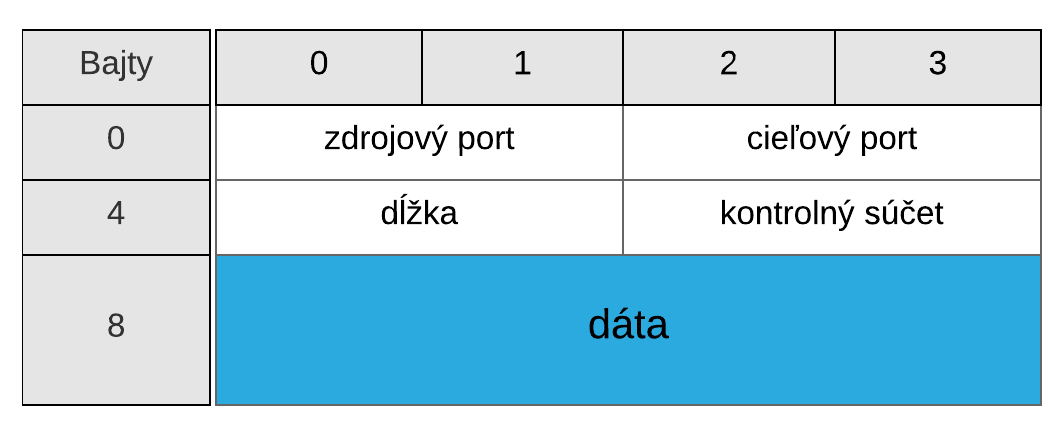
\includegraphics[width=.80\textwidth]{images/net-udp-head.png}
  \caption{Schéma popisujúca štruktúru UDP hlavičky a informácií}
  \label{fig:net-udp-head}
\end{figure}

Napriek tomu, že tieto dva protokoly sú pomerne odlišné a slúžia na rôzne
účely, ich spoločnou funkcionalitou je použitie portov pre identifikáciu
aplikácií komunikujúcich strán. Porty pre TCP a UDP sú na sebe navzájom
nezávislé, čo prináša možnosť komunikácie jedného zariadenie zároveň v TCP aj
UDP kontexte.

\section{Sieťová vrstva}
Sieťová vrstva je skupina internetových metód, protokolov a špecifikácií, ktorá
v sieťovom modely TCP/IP slúži (transportnej vrstve) na prenos datagramov
(paketov) od odosielateľa, cez jednotlivé sieťové rozhrania až k príjemcovi.
Každý z uzlov v sieti je na sieťovej vrstve identifikovaný takzvanou IP
\textit{(Internte Protocol)} adresou. Táto vrstva teda odvodzuje svoj názov od
svojej hlavnej funkcionality, ktorou je formovanie a tvorba pripojenia k
internetovej sieti prostredníctvom navzájom prepojených uzlov.

Protokoly sieťovej vrstvy pracujú s paketmi založenými na IP adresách
jednotlivých zariadení. Jednoznačne najznámejším protokolom tejto vrstvy je už
spomínaný IP \textit{(Internte Protocol)}, sieťová vrstva však definuje aj iné
dôležite protokoly ako napríklad: ICMP
\textit{(Internet Control Message Protocol)}, ktorý slúži na odosielanie
chybových správ operačnými systémami, alebo IGMP
\textit{(Internet Group Management Protocol)}pre podporu multicastu smerovačov.
Sieťová vrstva však neobsahuje žiadne protokoly, ktoré definujú komunikáciu na
úrovni lokálnej podsiete a fyzických spojení.

\subsection{Protokol IP}
IP protokol sieťovej vrstvy je zodpovedný za adresáciu hostiteľského uzlu a
prenos datagramu (paketu) od odosielateľa k príjemcovi cez jednu, alebo viacero
IP sietí. Pre tento účel definuje IP vlastný formát hlavičky paketov, čím
poskytuje logiku jednoznačnej identifikácie v rámci siete. Štruktúru hlavičky
IP paketu znázorňuje nasledujúci diagram.

\begin{figure}[h]
  \centering
    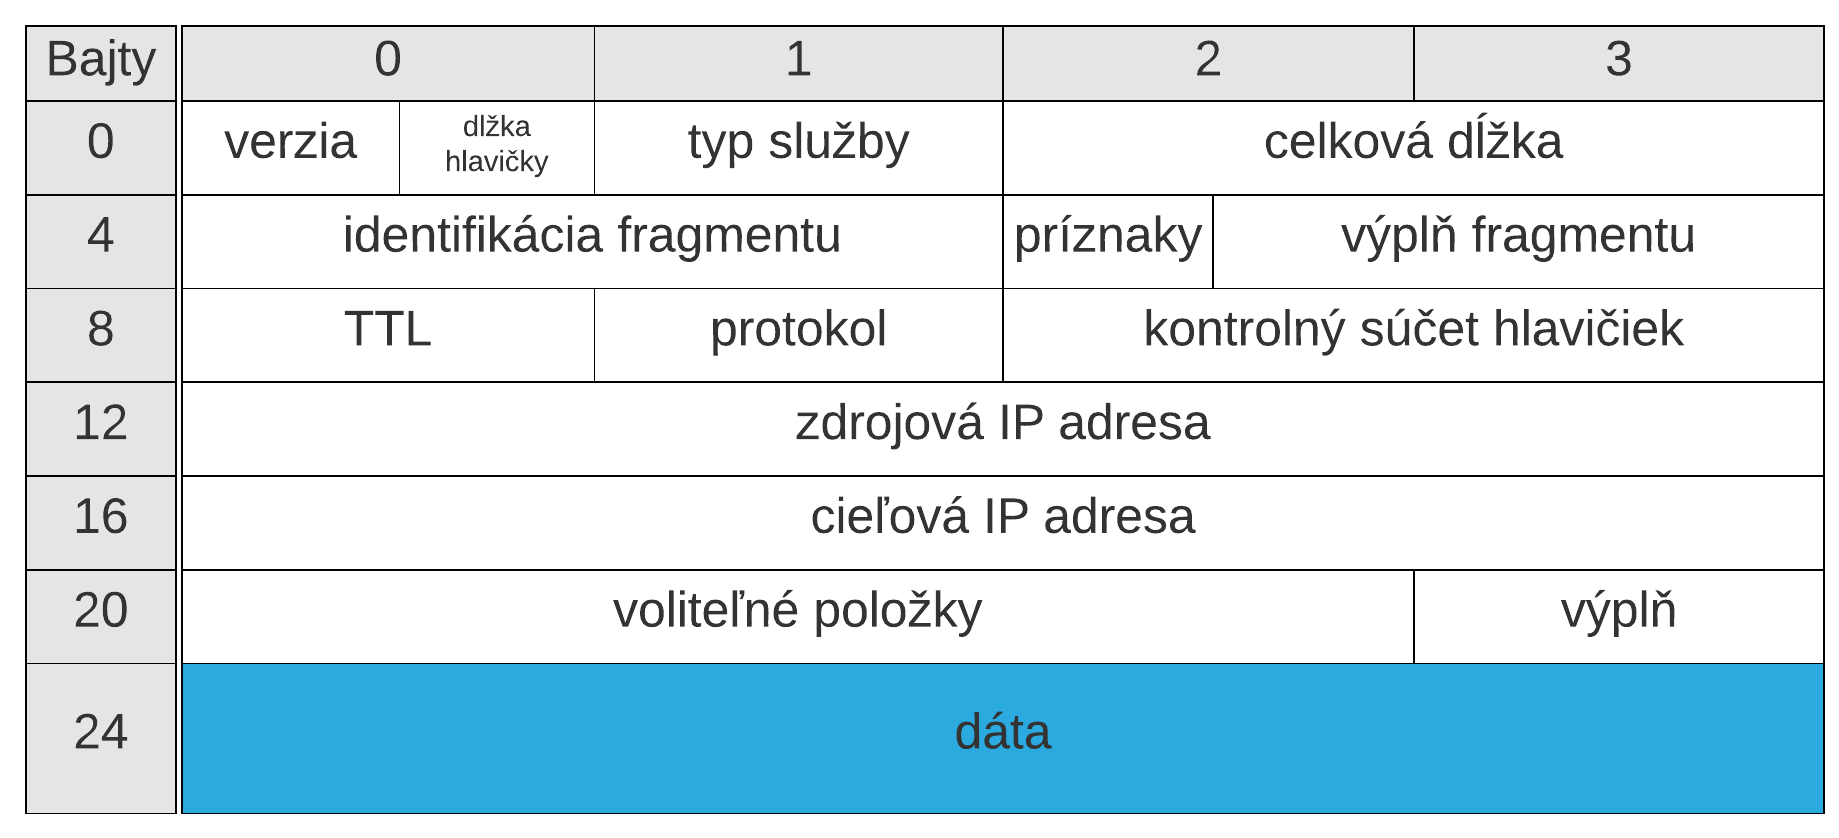
\includegraphics[width=.80\textwidth]{images/net-ip-head.png}
  \caption{Schéma popisujúca štruktúru hlavičky IP protokolu}
  \label{fig:net-ip-head}
\end{figure}

Zrejme najzaujímavejšou informáciu z hľadiska identifikácie bude samotná IP
adresa, ktorá okrem identifikácie zariadenia poskytuje aj informáciu o
približnej polohe uzlu ktorému bola priradené. Podrobne sa problematike
identifikácie pomocou IP adries venuje kapitola \ref{ch:existing}. 

V skutočnosti existujú dve verzie IP protokolu: IP verzie 4 a IP verzie 6.
Každá z týchto verzií definuje štruktúru IP adries rozdielne. IP adresy v IPv4
sú 32 bitové, čo obmedzuje ich počet na približne 4,2 miliardy adries. Z tohto
počtu sú niektoré konkrétne adresy rezervované na špeciálne účely ako napríklad
privátne siete (~18 miliónov adries), alebo adresy určené pre multicast
(~270 miliónov). Rapídny pokles počtu voľných IPv4 adries preto vyústil do
rozšírenia protokolu o IPv6. IPv6 definuje 128 bitové adresy, z čoho vyplýva,
že poskytne 3.4x1038 adries. Tento počet by mal byť do budúcna viac ako
dostačujúci.

\section{Vrstva sieťového rozhrania}
Vrstva sieťového rozhrania funguje v TCP/IP modeli na najnižšej úrovni.
Táto vrstva popisuje samotnú sieťovú architektúru a jej komunikáciu na úrovni
fyzického pripojenia. Ide o skupinu metód a komunikačných protokolov, ktoré 
teda operujú na fyzickom spojení dvoch uzlov.

Niektorými z jej dôležitých protokolov sú: ARP
\textit{(Address Resolution Protocol)}, RARP
\textit{(Reverse Address Resolution Protocol)},
NDP \textit{(Neighbor Discovery Protocol)}, OSPF
\textit{(Open Shortest Path First)} a iné.

Informácie týchto protokolov však operujú na príliš nízkej úrovni sieťovej
infraštruktúry, preto ich nebude možné využiť pri identifikácií. V prehľade je 
teda vrstva sieťového rozhrania uvedené len pre úplnosť.

\chapter{Útoky typu \textit{Denial of Service}}
\label{ch:dos}
Jedným z hlavných dôvodov identifikácie užívateľov je prevencia proti útokom. Medzi
najznámejšie z útokov patrí tzv. \textit{Denial of Service}, ďalej len \textit{DoS}.

Vo všeobecnosti je za \textit{DoS} útok považovaná snaha útočníka zabrániť oprávneným
užívateľom v prístupe k informáciám, prípadne službám poskytovateľa. Snahou útočníka
je znefunkčniť pripojenie neustálym narúšaním služby serveru, prípadne sieťovej
infraštruktúry, v dôsledku čoho môže dôjsť k čiastočnej, či úplnej strate
internetového pripojenia hostiteľa. 

\begin{figure}[h]
  \centering
    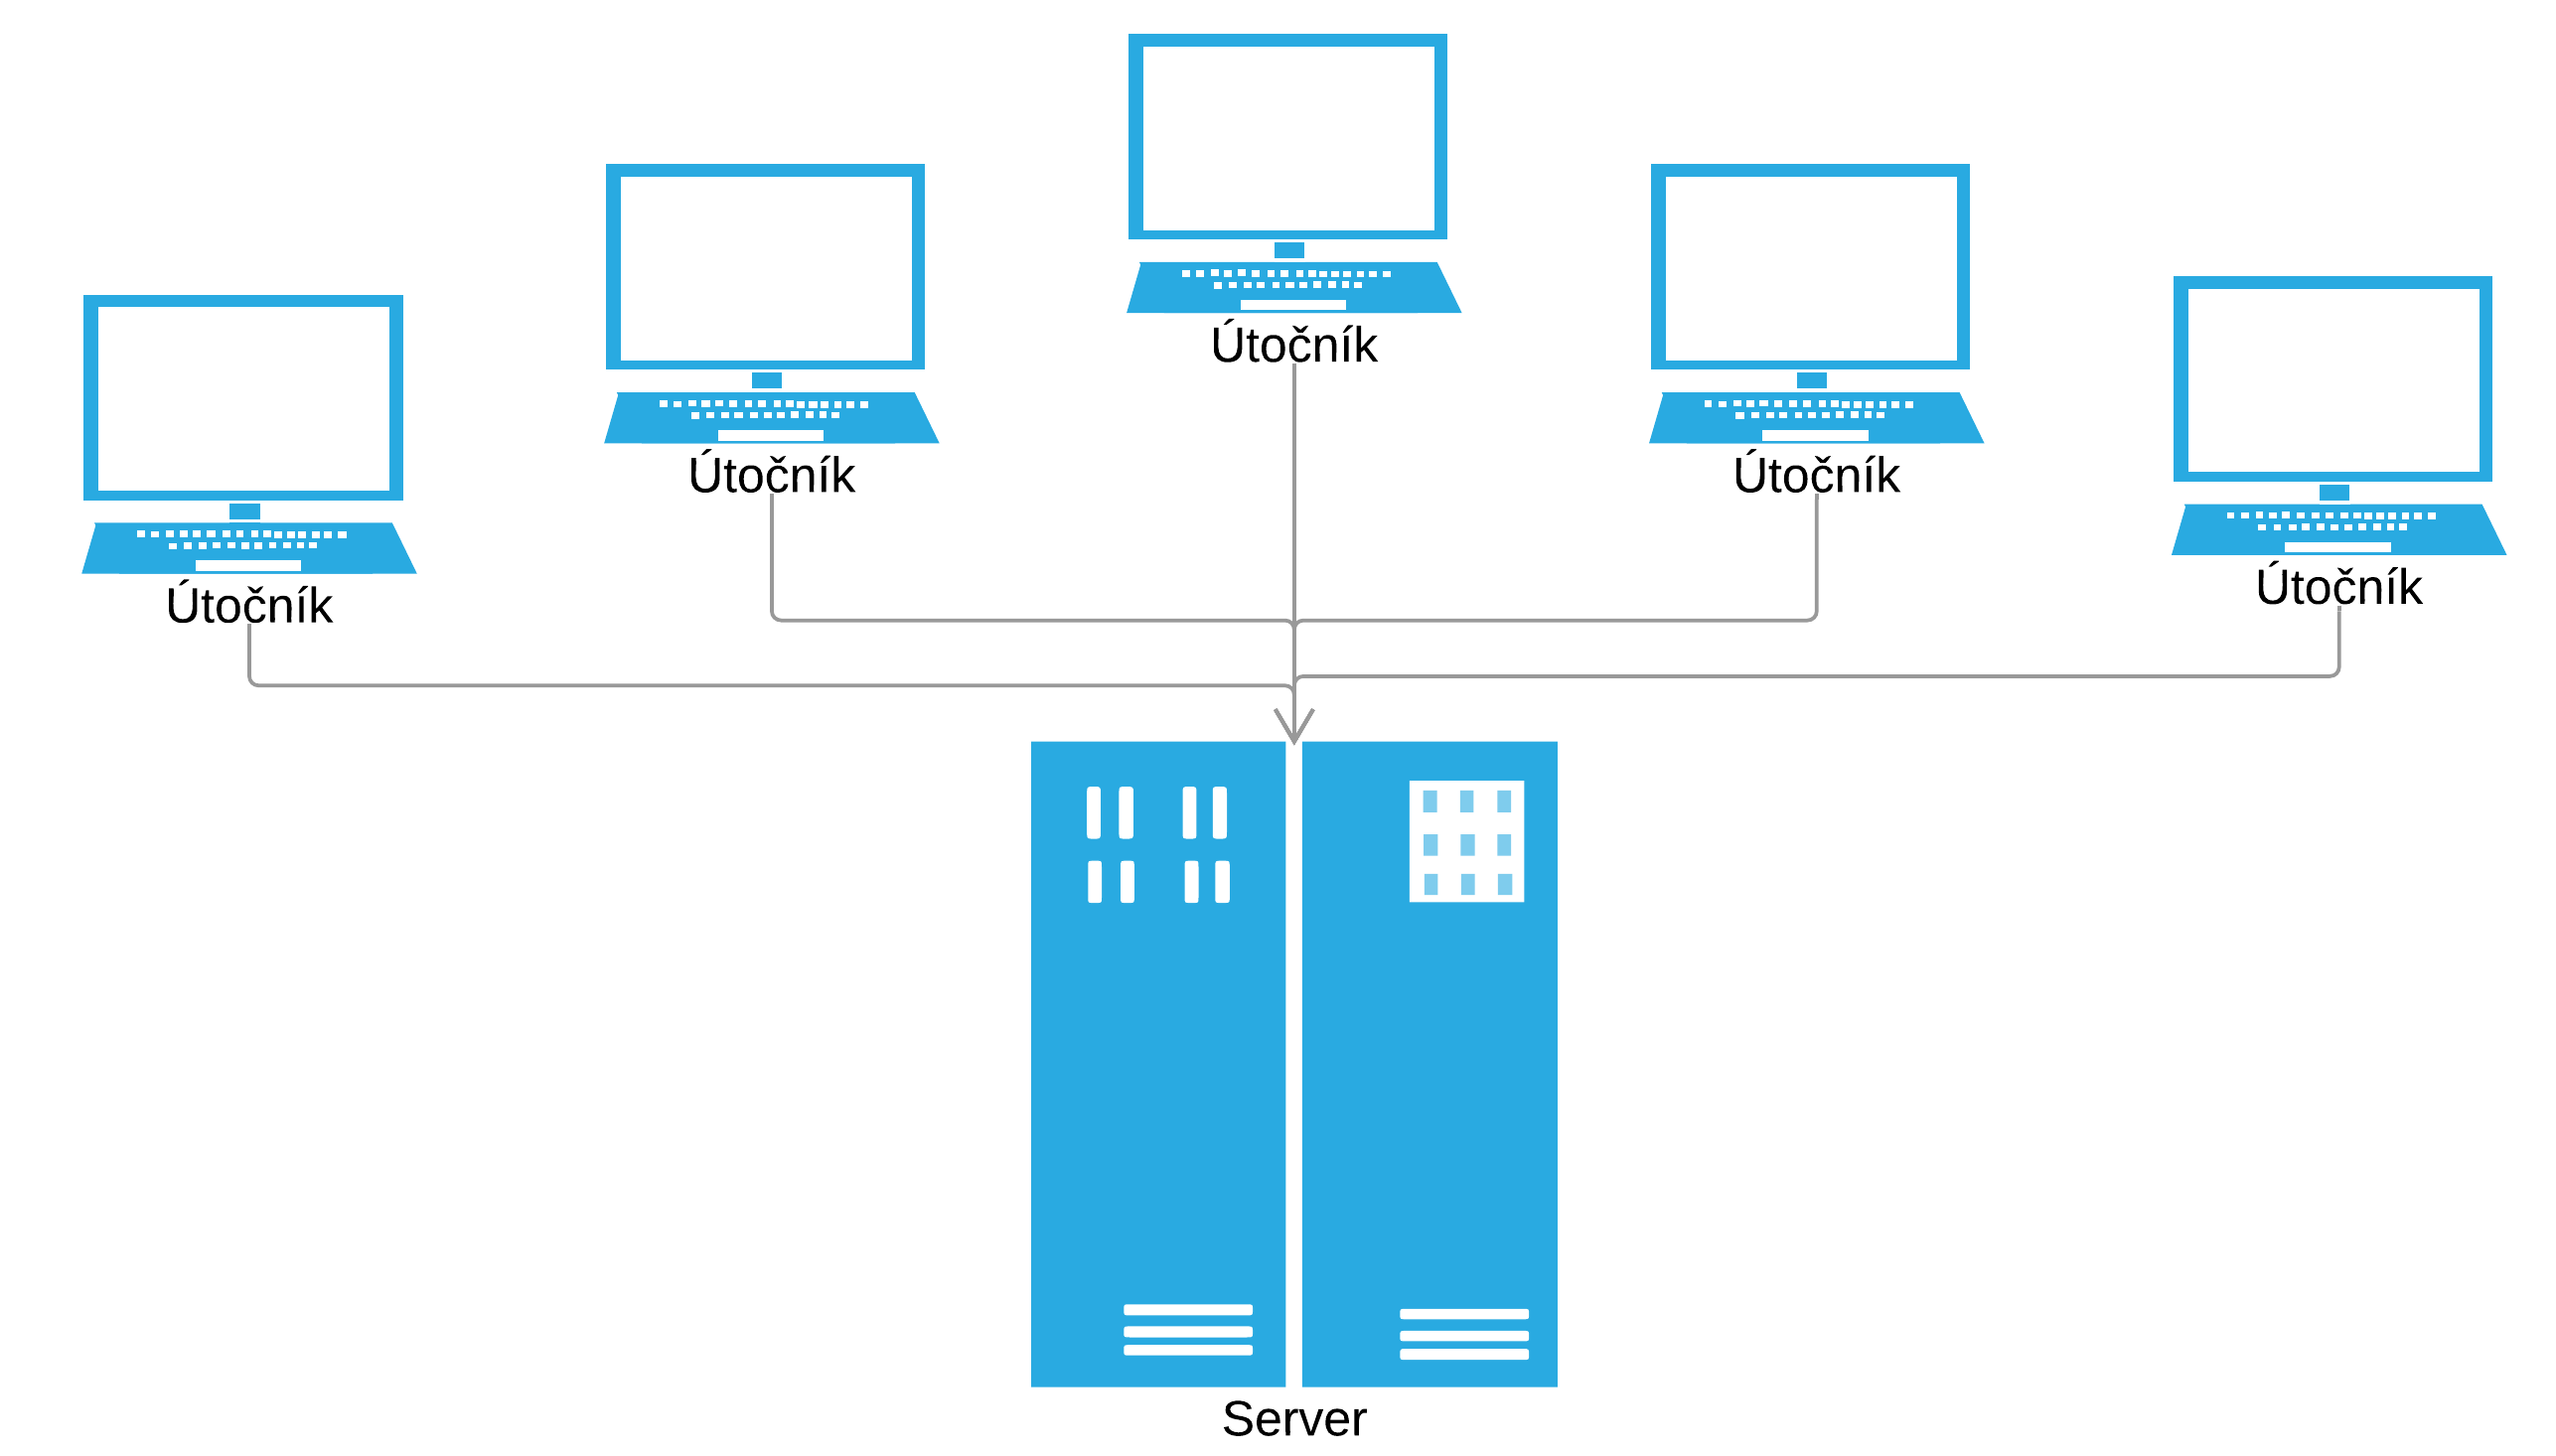
\includegraphics[width=\textwidth]{images/dos.png}
  \caption{Schéma DoS útoku, zdroj: vlastné spracovanie}
  \label{fig:cs-basic}
\end{figure}

U distribuovaného \textit{DoS} útoku môže útočník použiť k útoku na server
počítače klientov. Nad týmito zariadeniami je možné prevziať kontrolu využitím
bezpečnostných chýb alebo nedostatkov. Takto je následne možné donútiť počítač
posielať obrovské množstvo dát na webové servery, prípadne odosielanie nevyžiadanej
pošty na konkrétne e-mailové adresy. Útok sa nazýva "distribuovaný", pretože útočník
používa viac zariadení na začatie útoku \textit{denial-of-service}.

\textit{DoS} útok je podobný veľkej skupine ľudí, ktorá sa zhromažďuje pri vstupe do
obchodu a bráni vo vstupe skutočným zákazníkom, ktorých záujmom sú reálne služby.
Útočníci vykonávajúci tieto útoky sa často zameriavajú na webové služby a servery,
ktoré sú poskytované vysoko profitujúcimi inštitúciami, ako sú napríklad banky,
prípadne platobné brány.

\section{Základne typy a techniky}
Nasledujúce odseky popisujú najpoužívanejšie typy a techniky vykonávania \textit{DoS}
útokov a identifikujú prostriedky, ktorými je im možné zabrániť.

\subsection{Distribuované DoS útoky}
O distribuovaných \textit{DoS} útokoch hovoríme v prípade, že viaceré zariadenia zaplavia
celú šírku pásma prípadne zdrojov cieľového systému, ktorým je zvyčajne jeden, alebo viacero
serverov. Takýto útok je často dôsledkom použitia rôznych systémov a zariadení (napríklad
\textit{botnetu}), ktoré sa snažia vyťažiť cieľový systém. \textit{Botnet} je rozsiahla
virtuálna sieť umelých (\textit{zombie}) počítačov, ktorých cieľom je prijímať príkazy bez
vedomia majiteľa. Keď cieľový systém spotrebuje všetky voľné spojenia, ďalšie (nové) už nie
je možné nadviazať. Hlavné výhody útočníka pri využití Distribuovaného \textit{DoS} útoku
spočívajú v skutočnostiach, že viaceré zariadenia dokážu generovať väčšiu záťaž ako jedno,
pričom použitie množstva systémov zabezpečuje omnoho ťažšiu detekciu útočníka a správanie
sa každého z týchto zariadení je menej pozorovateľné čo sťažuje obranu voči útočníkovi.
Tieto výhody taktiež spôsobujú vývoj obranných mechanizmov. Na strane cieľového serveru už
nebude stačiť jednoduché zvýšenie šírky pásma nad hranicu momentálnej veľkosti útoku, pretože
útočník môže napríklad zvýšiť počet zapojených zariadení čím by taktiež spôsobil zaťaženie a
výpadok systému.

\begin{figure}[H]
  \centering
    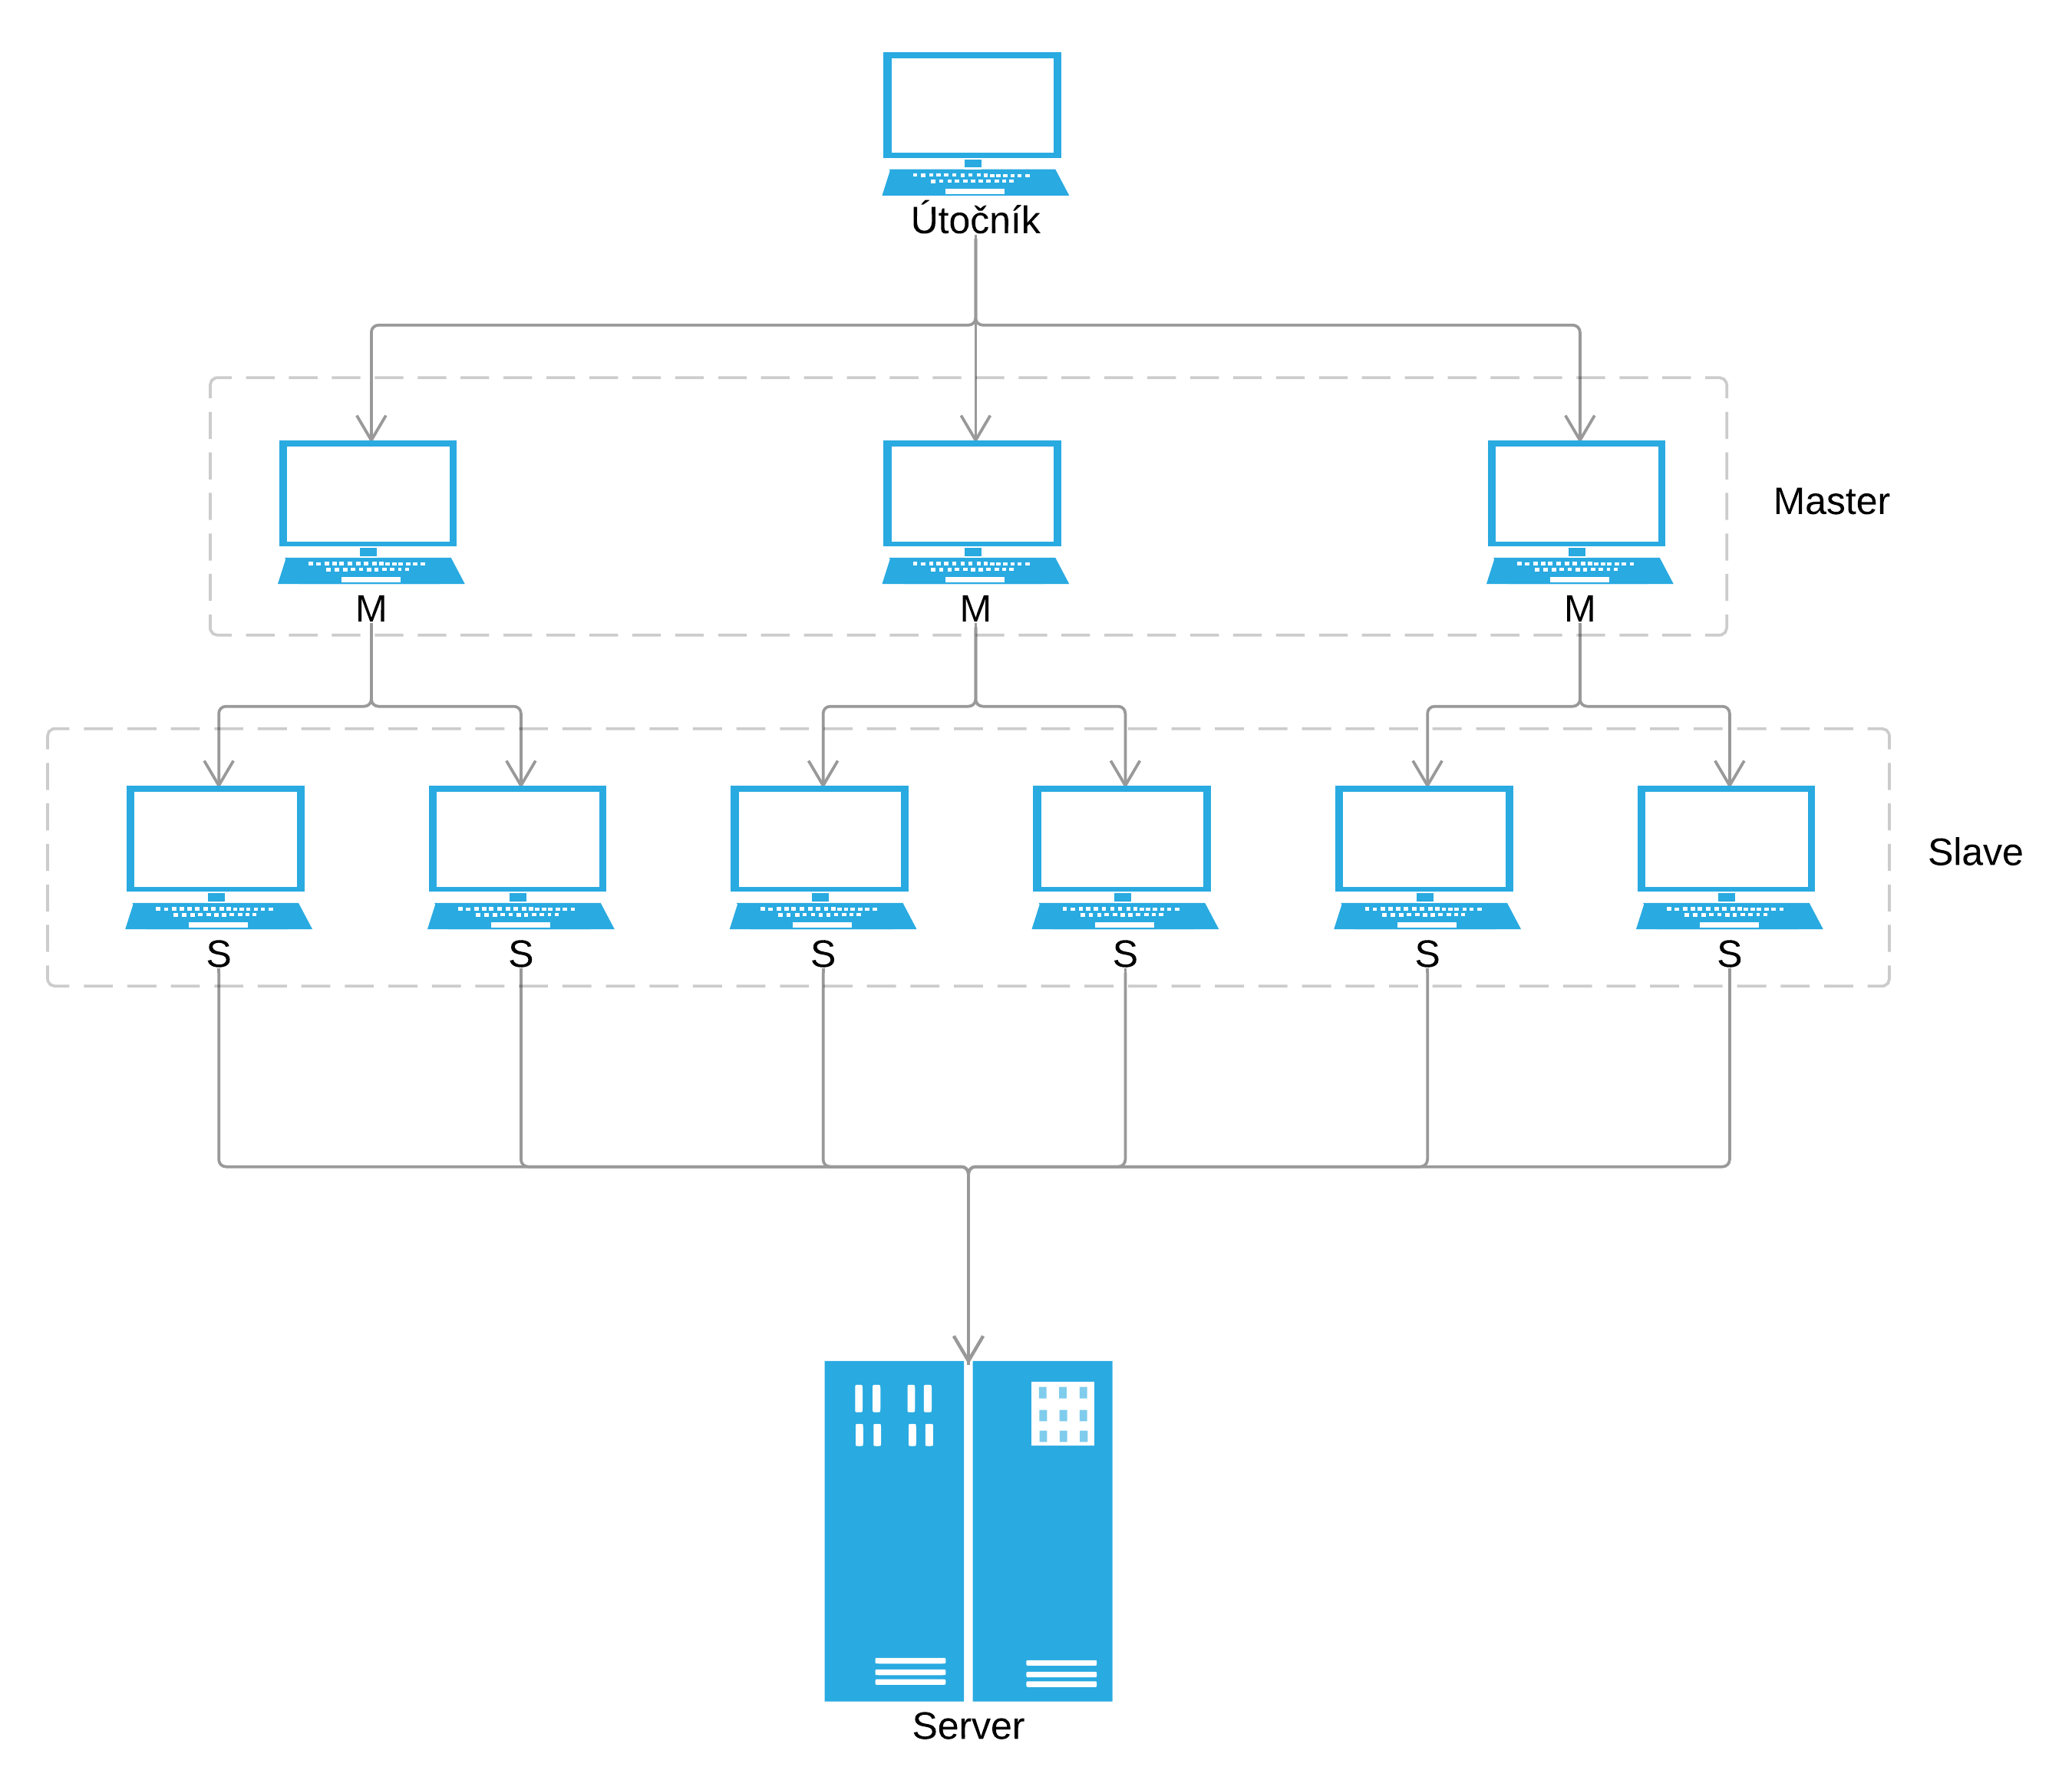
\includegraphics[width=\textwidth]{images/ddos.png}
  \caption{Schéma rozloženia DDoS útoku, zdroj: vlastné spracovanie}
  \label{fig:cs-basic}
\end{figure}

\subsection{Sémantické DoS útoky}
Sémantické útoky využívajú špecifickú funkcionalitu, alebo implementačnú chybu aplikácie,
prípadne protokolu zariadenia obete na zneužitie určitého množstva jeho zdrojov. Napríklad
v prípade \textit{TCP SYN} útoku je touto zneužitou funkcionalitou alokácia značného množstva
priestoru v zozname pripojení ihneď po potvrdení \textit{ TCP SYN requestu}. Útočník otvorí
viaceré spojenia, ktoré nikdy neuzavrie, čím zahlcuje server. 

Pri \textit{CGI} útoku je cieľom útočníka takýmto spôsobom zahltiť procesor viacerými
\textit{CGI requestami}.

Jedným z obzvlášť nebezpečných útokov je \textit{NAPTHA} útok, ktorý sa zameriava na
\textit{TCP} protokol. Inicializuje mnoho \textit{TCP} spojení, ktoré zaplnia zdroje serveru.

\subsection{Brute-force útoky}
TODO 

Source ref: https://www.eecis.udel.edu/~sunshine/publications/ccr.pdf

\subsection{Reflexia a zosilnenie}
TODO
% A reflector is any IP host that will return a packet if sent a packet. Attackers
% orchestrate the hosts under their control to send the spoofed traffic purportedly
% coming from the victim to reflectors. The result is that the flood at the
% victim arrives from a significantly higher number of sources, an exceedingly diffuse
% flood likely clogging every single path to the victim from the rest of the internet.

\begin{figure}[h]
  \centering
    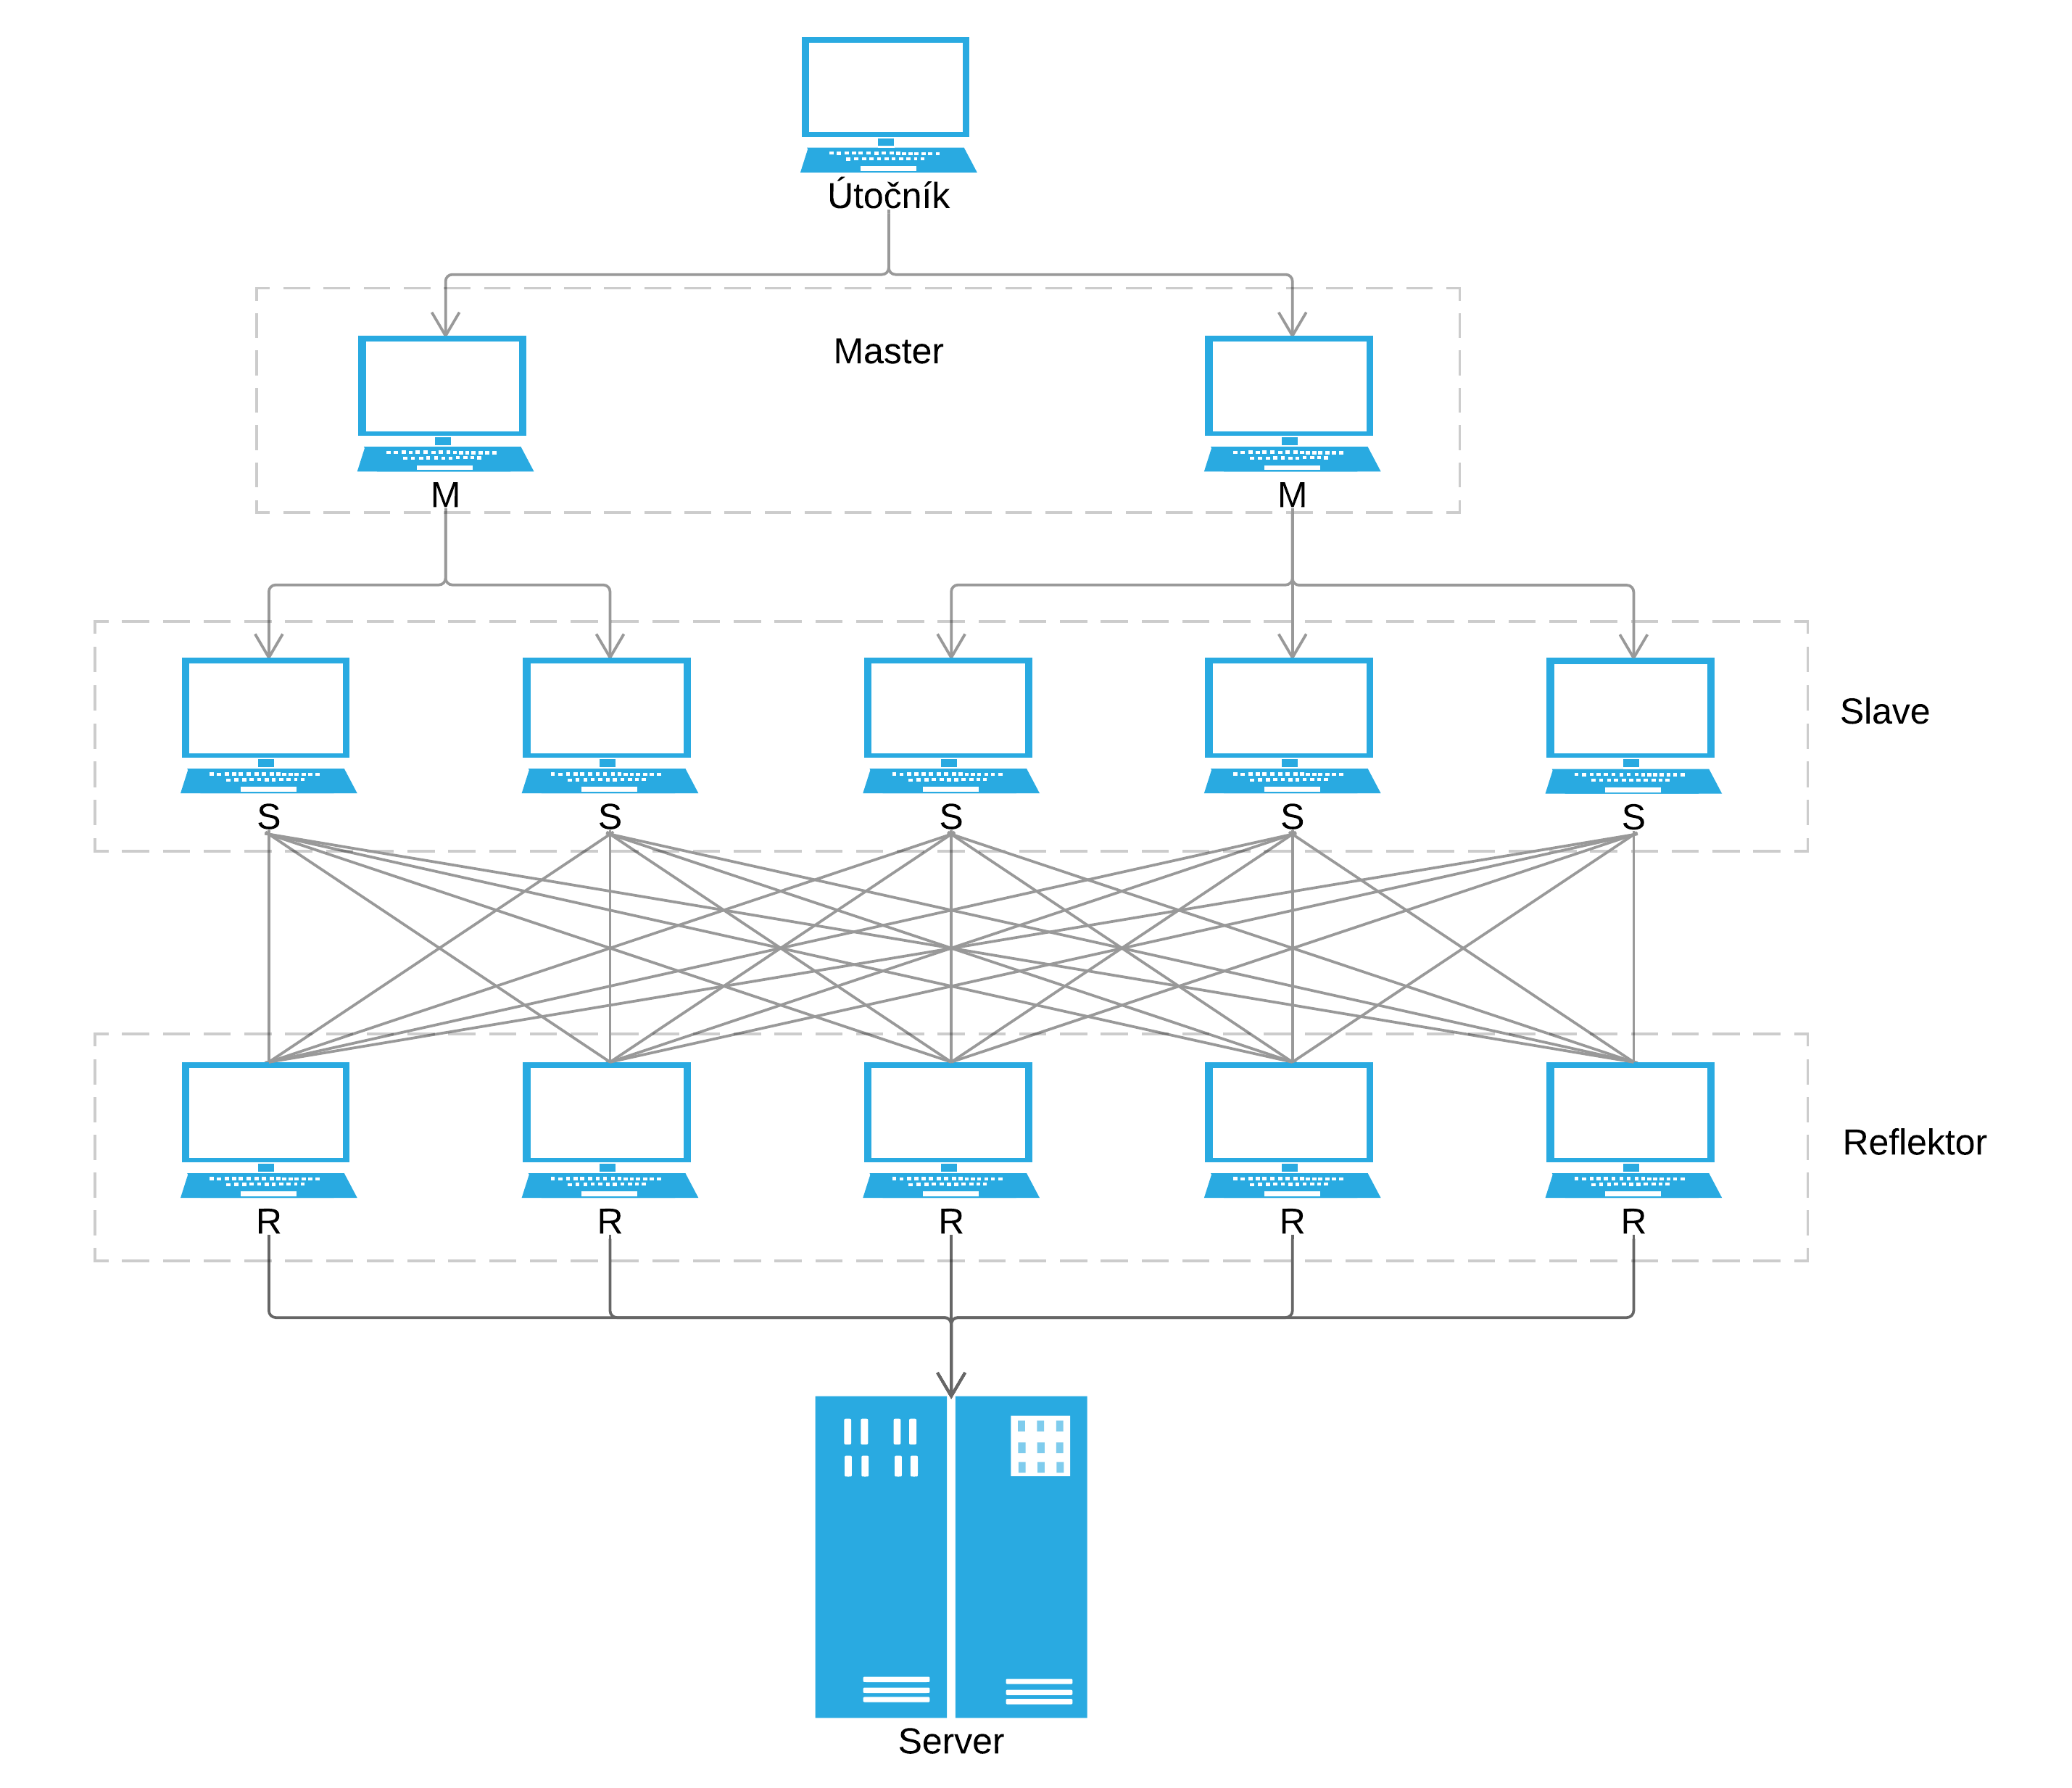
\includegraphics[width=\textwidth]{images/drdos.png}
  \caption{Schéma rozloženia DRDoS útoku, zdroj: vlastné spracovanie}
  \label{fig:cs-basic}
\end{figure}

% Amplification: An amplification attack is a type of the reflection attack in which
% reflectors’ responses are larger than queries. Therefore the volume of the attack
% traffic from the source to the victim is multiplied .

\subsection{HTTP POST DoS útoky}
TODO
% First discovered in 2009, the HTTP POST attack sends a complete, legitimate HTTP POST header, which includes a 'Content-Length' field to specify the size of the message body to follow. However, the attacker then proceeds to send the actual message body at an extremely slow rate (e.g. 1 byte/110 seconds). Due to the entire message being correct and complete, the target server will attempt to obey the 'Content-Length' field in the header, and wait for the entire body of the message to be transmitted, which can take a very long time. The attacker establishes hundreds or even thousands of such connections, until all resources for incoming connections on the server (the victim) are used up, hence making any further (including legitimate) connections impossible until all data has been sent. It is notable that unlike many other (D)DoS attacks, which try to subdue the server by overloading its network or CPU, a HTTP POST attack targets the logical resources of the victim, which means the victim would still have enough network bandwidth and processing power to operate. Further combined with the fact that Apache will, by default, accept requests up to 2GB in size, this attack can be particularly powerful. HTTP POST attacks are difficult to differentiate from legitimate connections, and are therefore able to bypass some protection systems. OWASP, an open source web application security project, has released a testing tool to test the security of servers against this type of attacks.

\section{DoS nástroje a DoS as a Service}
Typickou metódou prenosu mechanizmov \textit{DDoS} útokov je malvér. Jedným z príkladov bol
takzvaný \textit{MyDoom}. Ide o \textit{DoS} mechanizmus, ktorý sa spúšťal vo predom naplánovanom čase.
Tento útok zahŕňal nastavenie hodnoty \textit{IP} adresy cieľového systému pre nasadenie malvéru,
pričom pre spustenie útoku nebola potrebná žiadna interakcia s používateľom.

Ďalším spôsobom zneužitia systému pre \textit{DDoS} útok je použitie skrytej časti softvéru tretej
strany, ktorý umožní útočníkovi stiahnutie \textit{zombie} agenta, prípadne ho už softvér sám obsahuje.
Útočník môže preniknúť do systému taktiež pomocou automatizovaných nástrojov, ktoré zneužívajú chyby v
programoch počúvajúcich vzdialené pripojenia. Tento scenár zasahuje primárne systémy, ktoré sa správajú
ako webové servery. Typickým príkladom \textit{DDoS} nástroja z tejto oblasti je takzvaný
\textit{Stacheldraht}. \textit{Stacheldraht} využíva vrstevnatú štruktúru, v ktorej útočník používa
program klienta na pripojenie sa k \textit{handlerom}, ktoré sú zneužívané na prenos príkazov
k \textit{zombie} agentom. Agenti následne vykonávajú samotný \textit{DDoS} útok. Agenti sú cez handleri
zneužívané útočníkom za pomoci použitia automatizovaných algoritmov na vyhľadávanie zraniteľností v
programoch, ktoré prijímajú vzdialené pripojenia. Každý \textit{handler} je schopný kontrolovať až tisíc
agentov. 

DDoS nástroje ako \textit{Stacheldraht} stále používajú klasické \textit{DoS} metódy zamerané na
zosilnenie a podvrhovanie IP adries ako napríklad útok vyťaženia šírky pásma. Ďalšou z možností je
zahltenie zdrojov - \textit{SYN Flood} útok. Novšie nástroje používajú na \textit{DoS} útoky taktiež
\textit{DNS} servery.

Nástroje ako \textit{MyDoom} môžu byť použité voči ľubovoľnej IP adrese. Menej skúsení útočníci ich
používajú k znemožneniu dostupnosti populárnych a známych webových serverov. Naopak sofistikovanejší
útočníci používajú tieto nástroje na vydieranie, napríklad voči svojim obchodným protivníkom.

V niektorých prípadoch sa však môže zariadenie stať časťou \textit{DDoS} útoku zámerne - so súhlasom
majiteľa. Príkladom je distribuovaný útok \textit{Operation Payback} organizovaný skupinu
\textit{Anonymous}.

---

TODO DoSaaS
% The LOIC has typically been used in this way. Along with HOIC a wide variety of DDoS tools are available today, including paid and free versions, with different features available. There is an underground market for these in hacker related forums and IRC channels.

% UK's GCHQ has tools built for DDoS, named PREDATORS FACE and ROLLING THUNDER.

% Some vendors provide so-called "booter" or "stresser" services, which have simple web-based front ends, and accept payment over the web. Marketed and promoted as stress-testing tools, they can be used to perform unauthorized denial-of-service attacks, and allow technically unsophisticated attackers access to sophisticated attack tools without the need for the attacker to understand their use.

\section{DoS - Zhrnutie}
TODO
% Simple attacks such as SYN floods may appear with a wide range of source IP addresses, giving the appearance of a well distributed DoS. These flood attacks do not require completion of the TCP three way handshake and attempt to exhaust the destination SYN queue or the server bandwidth. Because the source IP addresses can be trivially spoofed, an attack could come from a limited set of sources, or may even originate from a single host. Stack enhancements such as syn cookies may be effective mitigation against SYN queue flooding, however complete bandwidth exhaustion may require involvement.

% If an attacker mounts an attack from a single host it would be classified as a DoS attack. In fact, any attack against availability would be classed as a denial-of-service attack. On the other hand, if an attacker uses many systems to simultaneously launch attacks against a remote host, this would be classified as a DDoS attack.

% It has been reported that there are new attacks from internet of things which have been involved in denial of service attacks. In one noted attack that was made peaked at around 20,000 requests per second which came from around 900 CCTV cameras.


\chapter{Existujúce prístupy k identifikácií}
\label{ch:existing}
Nasledujúca kapitola sa venuje popisu, porovnaniu a hodnoteniu existujúcich
prístupov, ktoré sú momentálne využívané na účely identifikácie používateľa.
Ide najmä o techniky využívajúce: protokoly sieťovej vrstvy (najmä IP adresy),
monitorovanie TCP komunikácie a vlastné aplikačné identifikátory.

\section{Využitie sieťovej vrstvy}
Jedným z najtypickejších spôsobov identifikácie užívateľa a jeho zriadenia je
IP protokol sieťovej vrstvy. Táto technika je veľmi rozšírená napríklad pre
účely blokovania prístupu na server u systémových \textit{firewallov} a
podobne.
TODO - rozšíriť

\subsection{Internet Protocol (IP)}
Ako popisuje kapitola \ref{ch:net-layers}, Internet Protocol slúži na prenos
paketov medzi jednotlivými sieťovými uzlami - zariadeniami, ktoré sú
identifikované IP adresami. V ideálnom by bolo každé zariadenie v sieti
identifikované jednou statickou IP adresou. Bolo by teda možné užívateľa
rozpoznať len na základe množiny jeho adries. Bohužiaľ adresový priestor
protokolu IPv4 je obmedzený na 3.7 miliardy verejne dostupných adries
\footnote{
  Uvedené množstvo zahŕňa všetky možné dostupné IPv4 adresy - približne 4.2
  miliardy po odpočítaní rezervovaných adries - 588 miliónov.
}.
Z toho vyplýva potreba metód ich dynamického prideľovania, proxy serverov a
prekladu, čo identifikáciu značne komplikuje.

U dynamického prideľovania adries ide o jednoduché mapovanie pre zariadenia
na úrovni smerovača. Identifikácia je teda stále možná, len sťažená o vyšší
počet možných adries pre jedno zariadenie.

Preklad (\textit{Network Address Translation} IP adries však identifikáciu
prakticky znemožňuje. Vo všeobecnosti ide o techniku prekladu jednej podmnožiny
IP adries na inú pomocou zmeny informácie o sieťovej adrese v datagrame IP
protokolu. Pôvodne sa táto technika používala pre zjednodušenie presmerovania
komunikácie bez nutnosti opätovnej adresácie každého uzlu. V pokročilých
implementáciách však dnes \textit{NAT} predstavuje veľmi populárnu možnosť
takzvaného  IP maskovania. Maskoavanie IP adries je technika zdieľania jednej
verejnej IP adresy celou privátnou podsieťou. Adresný priestor privátnej
podsiete, ktorá má byť skrytá je teda vždy mapovaný na verejnú IP adresu
smerovača. Táto adresa samotná je taktiež zvyčajne súčasťou väčšej podmnožiny
adresného priestoru. Pojem prekladu (\textit{NAT}) IP adries sa dnes už stal
synonymom ich maskovania. Paket odoslaný zo zariadenia, ktoré je prekryté
\textit{NAT} smerovačom bude teda ako zdrojovú adresu niesť namiesto IP adresy
zariadenia z ktorého pochádza hodnotu verejnej IP adresy smerovača.
Identifikácia na základe IP adresy preto v tomto prípade stráca význam.

\begin{figure}[h]
  \centering
    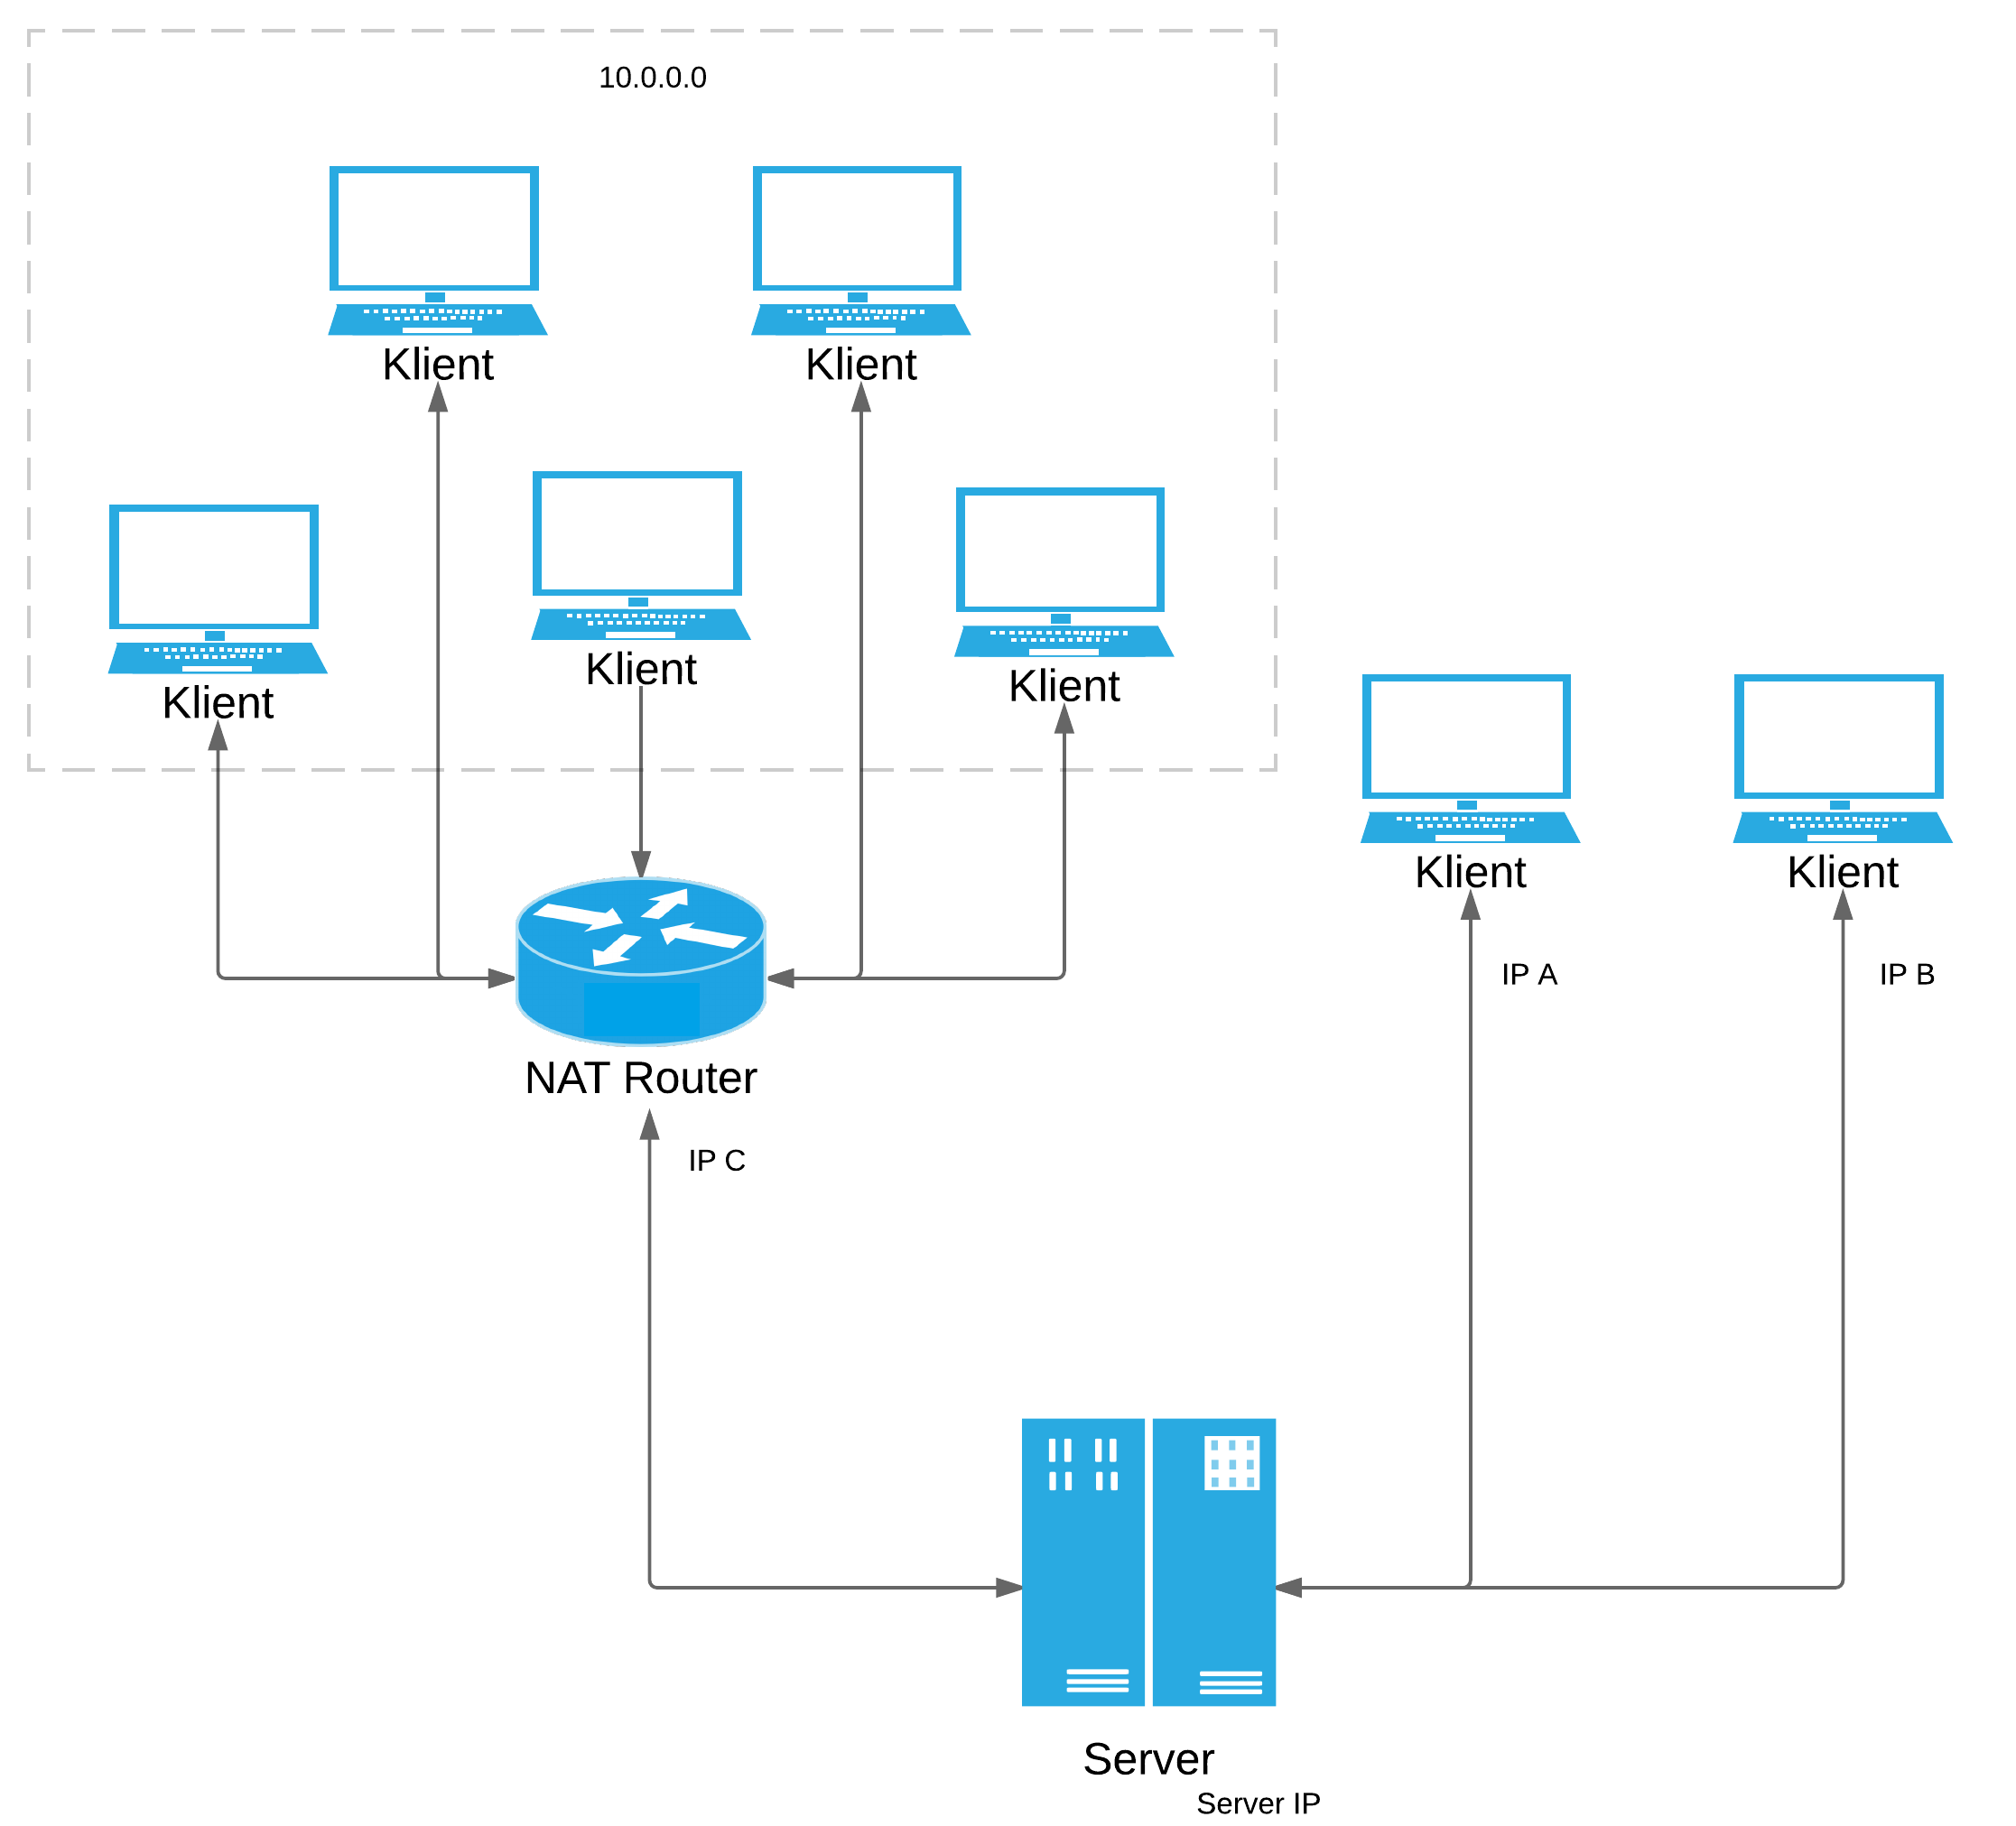
\includegraphics[width=.99\textwidth]{images/tech-IP-NAT.png}
  \caption{Vizualizácia rozloženia IP adresového priestoru pri použití techniky
  prekladu \textit{NAT}, zdroj: vlastné spracovanie}
  \label{fig:tech-IP-NAT}
\end{figure}

\subsection{Výhody a nevýhody}
Hlavnými výhodami použitia IP adries sú jednoduchosť, rýchlosť a flexibilita.
Napríklad pre účely znemožnenia prístupu stačí filtrovať len povolené IP
adresy, prípadne neumožniť prístup tým zakázaným. Oba spôsoby sú technicky veľmi
ľahko implementovateľné.

Ich nevýhodou je najmä rastúci trend použitia proxy serverov a \textit{NAT}
prekladu, čo má napríklad pri banovaní za následok znemožnenie prístupu aj
užívateľom, u ktorých to nie je potrebné, ale stoja za rovnakou IP adresou.

Vo všeobecnosti je teda identifikácia zariadení používateľa na základe IP
adresy možná. V prípade, že sa však zariadenie skrýva za proxy serverom,
prípadne sú adresy prekryté \textit{NATom} bude táto technika viesť takisto k
prekrytiu jednotlivých užívateľov v rámci podsiete.

\section{Monitoring TCP}
Ako popisuje predchádzajúca kapitola, TCP
\textit{(Transmission Control Protocol)} je jedným z protokolov transportnej
vrstvy sieťovej hierarchie. Jeho najtypickejším znakom je na rozdiel
od UDP garancia spoľahlivého doručenia paketov v presnom poradí. Prijatie
každého z paketov musí byť potvrdené príjemcom, inak je paket odoslaný znovu.
Poradie jednotlivých paketov je zaručené ich sekvenčnými číslami. Tieto 
vlastnosti robia z TCP jasnú voľbu pre aplikácie, ktoré vyžadujú nulovú
stratovosť dát. Aplikácie typicky zasielajú na TCP vrstvu \textit{stream} dát
pomocou takzvaných \textit{stream socketov}, čím sú dáta \textit{streamu}
rozdelené na primerane veľké segmenty. K segmentom je zároveň spočítaný
kontrolný súčet \textit{(TCP checksum)}, pomocou ktorého je možné určiť či
dáta neobsahujú poškodené pakety. Kontrolné súčty však nie sú v žiadnom ohľade
kryptograficky zabezpečené. Podrobný popis štruktúry TCP paketu znázorňuje
==obrazok kapitola 2?==

//TODO dokončiť
%Identifiers and their uniqueness
%The TCP protocol itself contains no data which can be used to identify a user (except such information is contained within the (unencrypted) data part of the packet). In addition to the lower level IP protocol, this is not true any more. The source and destination ports in cooperation with the IP address of the sender and receiver can identify both participating parties. 
%TCP is a good example for identifying information introduced by the “protocol obscurities” as described in Section 2.2 Although the meaning of the Sequence number field is defined – the initial value is not. It is up to the implementer how the initial sequence number is chosen (e.g., randomly). The same is true for instance for the Window field used for congestion control. As the congestion control has a key influence on the overall performance of TCP, many attempts to optimise them are done e.g., by operating system manufactures. 
%All these implementation depended information could be used for so called TCP/IP stack fingerprinting. The goal is to guess which TCP/IP stack and operating system is running on a remote machine. TCP/IP fingerprinting (as many other fingerprinting methods) can be done actively or passively; observing or modifying. A passive observing attempt would just listen on the networks links and tries to guess the TCP/IP stack from the eavesdropped data packets. An active observing attempt would also send data packets. The attacker would intelligently choose the data packets he sends to concluded as much information as possible from the remote host. But as it is still an observing attack the attacker would behave according to the protocol. Of course he could also violate the protocol rules. This typically gives him more possibilities for guessing the TCP/IP stack – but would make his attack also more obvious. 
%The software Nmap (“Network Mapper”) is a well-known representative for tools which are able to do TCP/IP fingerprinting. According to the developers, Nmap currently has more than 1500 fingerprints in its database.
%Of course the identifying information described above cannot only be used to guess the TCP/IP stack and operating system used but can also be used to link different TCP connections, especially if the guessed TCP/IP stack or operating system is a rather unusual one. Note that the information mentioned above can also be used to decide if TCP packets belong to the same TCP stream or not. Imagine for instance the situation that an attacker can monitor network traffic on different locations of the network whilst he cannot easily “follow” the TCP packets as an anonymisation service (operating at the IP layer) is used by the communication partners. Nevertheless chances are high that the attacker can still conclude who is communicating with whom just by looking at the TCP information. 
 
%Personal data
%The ports can leak information about the application used without looking at the data content. This is possible since there are standard ports used in the Internet, like port 25 for FTP, or port 80 for HTTP requests. If an application uses the Options field, this can contain personal information too, but this is very unlikely, since most application will use the Data field for such information. The Data field therefore can contain the most sensitive information, i.e., the application data.

\subsection{Vyhody a nevyhody}
TODO

\section{Aplikačné identifikátory}
Na aplikačnej úrovni je identifikácia užívateľa oveľa komplexnejším a do istej
miery aj abstraktnejším procesom. Z pohľadu systému sú jeho používateľmi
typicky ľudia, prípadne procesy iných služieb, ktoré existujú mimo neho.
Identifikátorom (ďalej len ID) užívateľa je teda projekcia aktuálneho
jednotlivca, prípadne procesu do počítačového systému. Systém používa typicky
abstraktný objekt - účet užívateľa, ktorý obsahuje množinu atribútov pre
každého jednotlivca, prípadne proces. Tento objekt má jednoznačné a unikátne
ID, prípadne meno, ktorým je reprezentovaný v rámci systému. Ďalej môže objekt
obsahovať dodatočné atribúty, ktoré ho popisujú. Atribúty môžu, ale nemusia
zahŕňať osobné údaje jednotlivca. Odhliadnuc od ID objektu, bezpečný systém
typicky priradí každému z používateľov jednoznačný identifikátor (číslo, alebo
reťazec), ktorým sa odkazuje na abstraktný objekt reprezentujúci aktuálnu
entitu. Tvorba unikátneho abstraktného objektu vo forme užívateľského účtu
pre každého jednotlivca, alebo proces komunikujúci so systémom je na aplikačnej
úrovni veľmi dôležitá. Tento objekt je následne používaný na identifikáciu
užívateľa v rámci celého systému. Zároveň tento objekt slúži ako odkaz pre
jednotlivé akcie systému umožňujúce prístup k údajom komunikujúcej entity.
ID používateľa sa tak stáva základom pre kontrolu prístupu. Z toho dôvodu je 
nevyhnutné uchovávať unikátne ID pre každého používateľa, keďže každý z nich
môže mať rozličné požiadavky a individuálne zodpovednosti v rámci akcií tohto
systému.

Metóda identifikácie systému poskytuje na aplikačnej úrovni jednoznačnú
identitu používateľa. Táto identita je typicky reprezentovaná jeho
identifikátorom. Systém preto prehľadáva všetky dostupné abstraktné objekty a
vráti objekt vyhovujúci privilégiám a atribútom entity s ktorou aktuálne
komunikuje. Po úspešnom dokončení tohto procesu je užívateľ jednoznačne
identifikovaný.

Po úspešnej identifikácií typicky nasleduje krok validácie získanej identity,
vo všeobecnosti nazývaný autentizácia používateľa. Fakt, že užívateľ tvrdí,
že je reprezentovaný špecifickým abstraktným objektom nemusí totiž nutne
znamenať, že je to pravda. Pre potvrdenie, že aktuálny používateľ môže byť
skutočne mapovaný na konkrétny abstraktný objekt, čim mu budú udelené jeho
práva a privilégiá musí komunikujúci preukázať svoju identitu systému.
Autentizácia je teda procesom validácie danej poskytnutej identity. Informácie,
ktoré predkladá komunikujúca entita sa nazývajú poverenia
(\textit{credentials}). Tieto poverenia sa môžu v rôznych systémoch líšiť, 
prípadne môžu niektoré systémy vyžadovať ich väčšie množstvo. Najčastejšími
formami týchto údajov sú: meno, heslo, pin, token, prípadne certifikáty, a iné.

Akonáhle prebehne úspešná autentizácia môže používateľ vykonať akcie, na ktoré
ma oprávnenia. Všetky akcie ktoré vykoná sú zviazané s jeho identitou a je ich
preto možné dodatočne trasovať.

\begin{figure}[h]
  \centering
    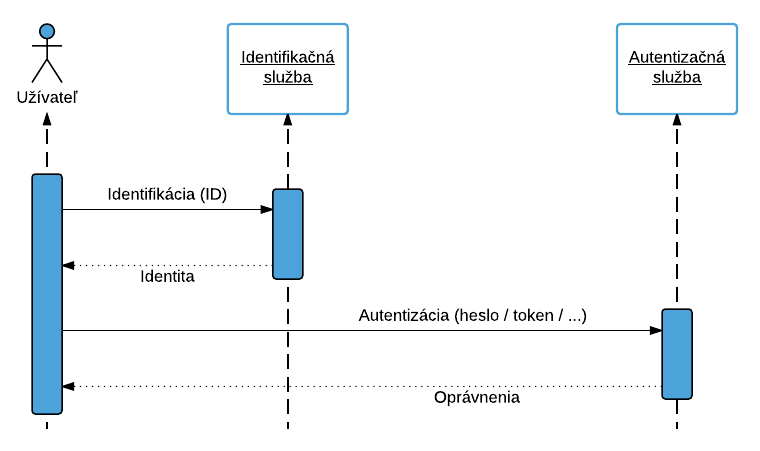
\includegraphics[width=.99\textwidth]{images/tech-app.png}
  \caption{Grafické znázornenie procesu identifikácie užívateľa na aplikačnej
  úrovni a jeho následnej autentizácie, zdroj: vlastné spracovanie}
  \label{fig:tech-app}
\end{figure}

\subsection{Výhody a nevýhody}
Identifikátory na aplikačnej úrovni sú veľmi jednoznačné a presné z hľadiska
priradenia účtu užívateľovi. Je pomocou nich preto následne možné presne
sledovať jeho akcie a manipulovať s privilégiami.

Tieto identifikátory sa však v abstrakcií komunikácie nachádzajú príliš vysoko,
preto nie je pomocou nich možné ovplyvniť napríklad DoS útoky popísané v
kapitole \ref{ch:dos}.

\section{Zhrnutie}
Na identifikáciu užívateľa, prípadne jeho zariadenia sú v súčasnosti
používané rôzne techniky na rôznych vrstvách sieťovej infraštruktúry. Od IP
adries sieťovej vrstvy cez atribúty TCP protokolu až po komplexné aplikačné
identifikátory. V praktickej časti tejto práce, ktorá sa zaoberá tvorbou
unikátneho identifikátoru, bude použitá kombinácia informácií zo všetkých
spomínaných vrstiev (IP adresy, informácie z HTTP a TCP protokolu, ...) tak,
aby vznikol čo najpresnejší možný odtlačok aktivity jedného užívateľa.

\chapter{Tvorba unikátneho identifikátoru}
\label{ch:footprint}
Hlavným cieľom a výstupom tejto práce je algoritmus definujúci jednoznačný
identifikátor užívateľa. Nasledujúca kapitola sa zaoberá práve popisom jeho
fungovania, štruktúty, použitých technológií a následnou implementáciou. Na
jeho tvorbu boli použité práve informácie HTTP a TCP protokolu popísané v
kapitolách \ref{ch:net-layers} a \ref{ch:existing}. Vďaka nim je algoritmus
schopný rozpoznať a priradiť aktivitu každému z používateľov hostiteľského
systému.

\section{Popis Algoritmu}
TODO

\section{Štruktúra identifikátoru}
TODO - Úvod

\subsection{Statické dáta}
TODO

\subsection{Relačné dáta}
TODO

\section{Algoritmus hľadania podobnosti}
TODO - Úvod

\subsection{Použité postupy}
TODO - Popis

\subsubsection{Jaccard index}
TODO

\subsubsection{Porovnávanie atribútov}
TODO

\subsection{Funkcia na výpočet vzdialenosti}
TODO

\section{Implementácia}
TODO - Úvod

\subsection{Použité technológie}
TODO

\subsection{Štruktúra a rozdelenie funkcionality}
TODO

\chapter{Test s reálnymi dátami}
\label{ch:data}
TODO

\chapter{Záver}
TODO

\makeatletter\thesis@blocks@clear\makeatother
\phantomsection %% Print the index and insert it into the
\addcontentsline{toc}{chapter}{\indexname} %% table of contents.
\printindex

\appendix %% Start the appendices.
\chapter{Príloha}
Appendices of thesis.

\end{document}
